%\documentclass[stu, 12pt]{apa7}
\documentclass[stu, 12pt, floatsintext]{apa7}
%\usepackage{fontspec}
%\setmainfont{Times New Roman} % Or your system's equivalent serif font
\usepackage[american]{babel}
\usepackage{csquotes}
\usepackage[style=apa, backend=biber]{biblatex}
%\usepackage[style=authoryear, backend=biber]{biblatex} % Changed from style=apa
\usepackage{float}
\usepackage{multicol}
\usepackage{hyperref} % nameref is bundled with hyperref
\usepackage{graphicx}   % Required for including images
\usepackage{subcaption} % Required for subfigures and subcaptions
%\usepackage{listings}
%\usepackage{xcolor}
\usepackage{array}
\usepackage{booktabs}
\usepackage{multirow}
\usepackage[dvipsnames]{xcolor}
\usepackage{amsmath}
\usepackage{amssymb}
\usepackage{enumitem,xcolor}

% Define the console style before using it
%\lstdefinestyle{console}{
	%	backgroundcolor=\color{black!5},
	%	basicstyle=\ttfamily\small,
	%	breaklines=true,
	%	frame=single,
	%	rulecolor=\color{black!30}
	%}
\graphicspath{
	{../img/}
	%   {../img_ipynb/}
	%	{../img/H1/}
	%	{../../results/DayResult/}
}
\DeclareGraphicsExtensions{.pdf,.jpeg,.png,.jpg}

\hypersetup{
	colorlinks=true,
	linkcolor=blue,
	citecolor=blue,
	urlcolor=blue
}

\addbibresource{../ref/references.bib}
\title{Agentic Fraud Detection via Dual-Threshold ML Classification\\and Generative Data Augmentation \& Benchmarking}
\author{Max Raxy}
\affiliation{Udacity Institute of AI \& Technology}
\course{Capstone-7: Integrative Industry Synthesis}
\professor{~}
\duedate{\today}

\begin{document}
	\maketitle
	\tableofcontents
	\newpage
	\listoffigures%\thispagestyle{fancy}
	\listoftables%\thispagestyle{fancy}
	\newpage

\section{Overview and Industry Context}
Credit card fraud detection is a critical challenge in the \textcolor{red}{\textbf{Financial Industry}}. Transactions are heavily imbalanced (e.g. less than 0.2\% fraudulent cases), making precise classification vital. False Negatives (FN) incur direct financial losses, charge-back fees, and reputational damage, while False Positives (FP) create customer friction and operational review costs. Balancing high recall with precision is essential for effective automated risk mitigation.

We are using \textbf{Credit Card Fraud Detection} dataset from \textbf{Kaggle}~\parencite{creditcardfraud}, which is an extremely imbalanced dataset with only 0.17\% in fraud-class . The goal is to use LangGraph~\parencite{langgraph_overview_2026} and develop an agentic workflow~\parencites{agentic_Plaat_2025}{agentic_Hughes04072025} to classify the transaction to Fraud and Not-Fraud (Legit). 

\section{Integration Rationale}
This project synthesizes three foundational capabilities (\textit{ML + GenAI + Agentic}), based on three previous projects :

\begin{enumerate}[font=\large\color{red}]
	\item\textbf{ Capstone-3:} Applied Machine Learning (Credit Card Fraud Detection)
	\begin{itemize}
		\item In Capstone-3, we avoid any oversampling and only use \textbf{cost-sensitive learning}~\parencites{cost-sensitive-learning1}{enwiki:cost-sensitive-learning2}
		\item Here, Transitioning from standard cost-sensitive learning to evaluate four oversampling methods for minority-class optimization.
	\end{itemize}
	\item \textbf{Capstone-5:} Generative AI Applications (Anime Face Generation with VAE)
	\begin{itemize}
		\item In Capstone-5, we developed Variational Auto-Encoder (VAE)~\parencites{org-vae1}{org-vae2} from scratch to generate new images
		\item Here, Adapting tabular-VAE (TVAE) and Conditional Tabular Generative Adversarial Networks (CTGAN)~\parencite{org-ctgan-tvae} from image generation to synthesize realistic tabular credit card transactions for data augmentation (oversampling) and benchmarking/testing.		
	\end{itemize}
	\item \textbf{Capstone-6:} Agentic AI Systems(Industrial Equipment Anomaly \& Incident Response Agent)
	\begin{itemize}
		\item In Capstone-6 we did not have real-dataset, and ML-classifier at initial stage (we used statistical threshold), and no vector database for historical context.
		\item Here, Upgrading prior heuristic-based anomaly response systems by integrating a trained ML classifier, vector database retrieval, to be used in  Retrieval-Augmented Generation (RAG)~\parencite{enwiki:rag}, and a multi-tiered escalation workflow.
	\end{itemize}
\end{enumerate}

\section{System Design and Technical Decisions}
The architecture employs an optimized dual-threshold ML classifier to handle high-certainty transactions directly, escalating ambiguous cases to a Large Language Model (LLM)~\parencite{enwiki:LLM} ReAct (Reasoning and Acting) agent~\parencite{react} using vector database~\parencite{enwiki:vector-db} historical context (RAG) saved in Long-Term Memory (LTM). Unresolved cases escalate further to human review as shown Fig.~\ref{fig:sys-block-diagram}.  The agentic system is built on top of three main parts (steps) as we will be explained in next sections.
\begin{figure}[H]
	\centering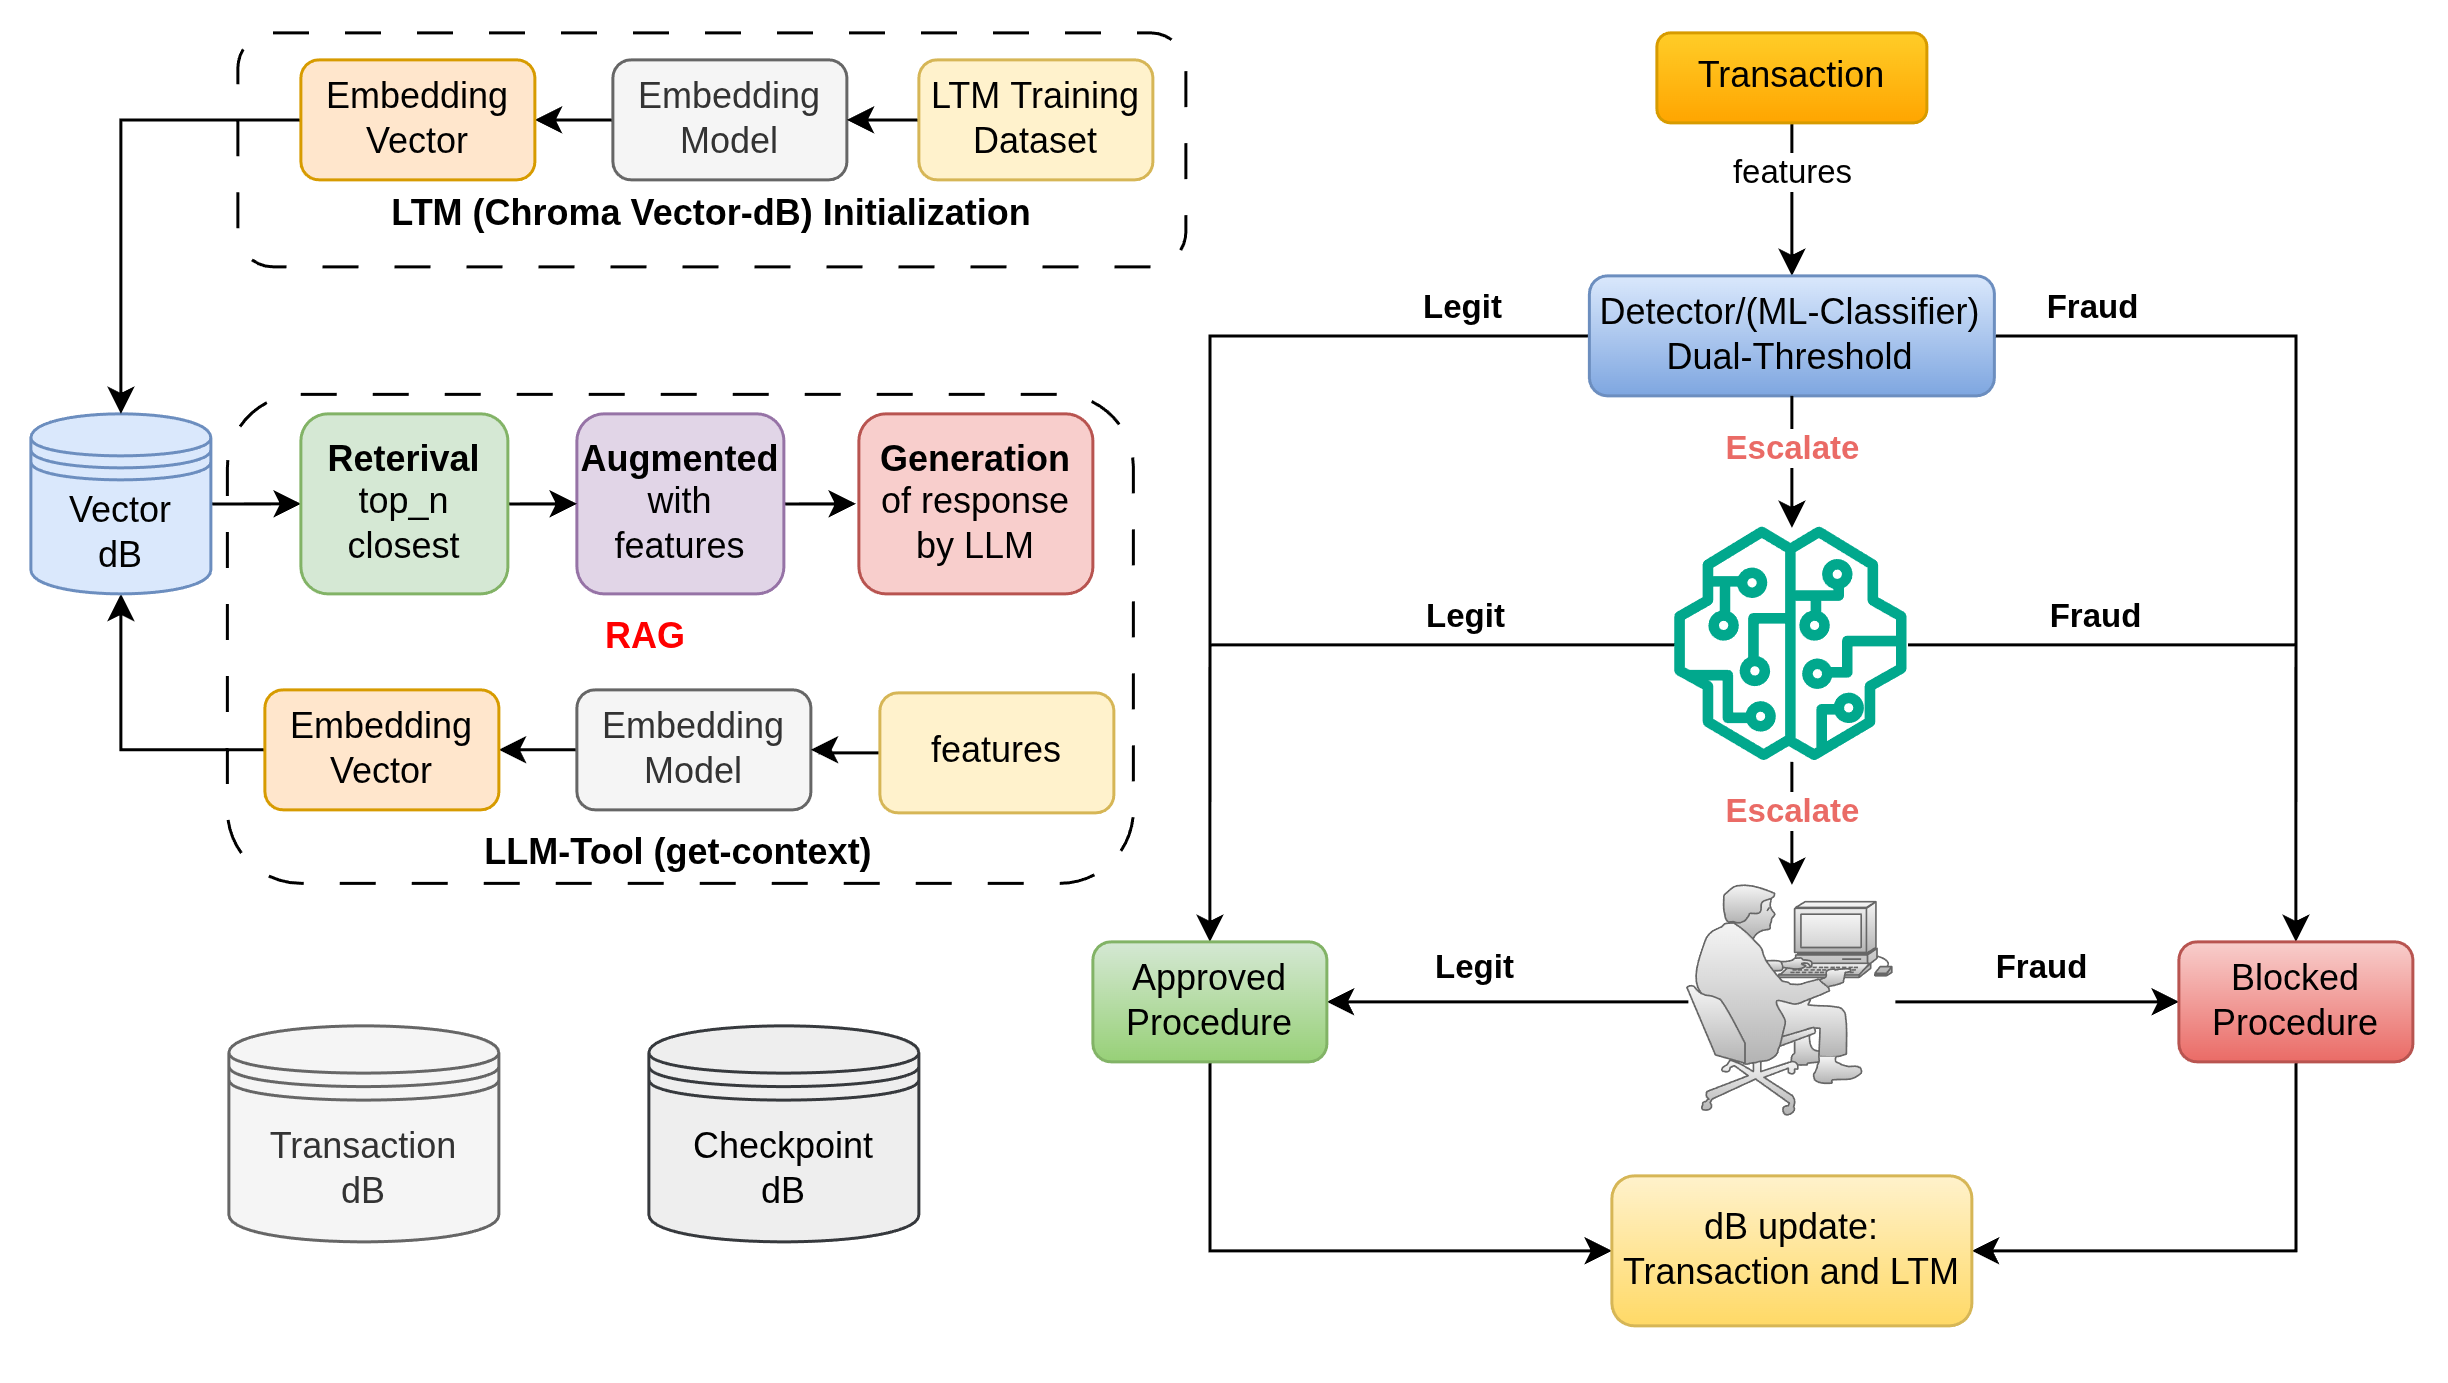
\includegraphics[width=1.0\textwidth]{agentic-block-diagram.drawio}
	\captionsetup{justification=centering}
	\caption{Agentic Workflow}
	\label{fig:sys-block-diagram}
\end{figure}

\subsection{Step-1: ML Classifier}
The following four over-sampling methods are used and evaluated using XGBoost as the base model in all cases (Note: XGBoost shows great performance for this dataset based on Capstone-3).
\begin{enumerate}[font=\large\color{red}]
	\item SMOTE (Synthetic Minority Over-sampling Technique)~\parencites{smote}{imb-learn}{imb-learn-doc}
	\item BSMOTE (BorderLine SMOTE)~\parencites{bsmote}{imb-learn}{imb-learn-doc}
	\item TVAE (Tabular VAE)~\parencites{org-ctgan-tvae}{sdv-paper}{sdv-git}
	\item CTGAN (Conditional Tabular GAN)~\parencites{org-ctgan-tvae}{sdv-paper}{sdv-git}
\end{enumerate}
TVAE/CTGAN needs training and since we have small number of sample to train these generative model we limit number of epoch to avoid over-fitting~\parencite{enwiki:overfitting}, and evaluate them based on final classification metrics like Precision/Recall~\parencite{enwiki:clf-metrics}, F-Score~\parencite{enwiki:f-score}, or Precision-Recall Area Under Curve (PR-AUC)~\parencite{mlm:pr-auc} .  Since  in credit card fraud  situation, FN can be more costly for the business and even have reputational damage consequence, we put more emphasize on Recall, and use F2-Score.

Performance comparisons are shown in Fig.~\ref{fig:model-perf-thr-inv} and Fig.~\ref{fig:model-best-thr}.  Model with CTGAN-augmented data is promising (PR-AUC=91.38\%, and F2-Score=90.23\%), and TVAE did not perform well in comparison (PR-AUC=87.06\%, and F2-Score=84.42\%). Also the model without oversampling (called XGB\_None) perform well based  on threshold invariant  metrics (PR-AUC=90.12\%), but when we use optimized threshold (based of F2-Score) , while it has highest precision (Precision=96.43\%) , does not have good  performance on recall (Recall=86.17\%).

Overall while the model without oversampling and adding any artificial minority samples perform well (as also discussed in Capstone-3), but using oversampling can improve the recall (XGB\_CTGAN-Recall = 90.43\% vs XGB\_None-Recall=86.17\%) and  overall F2-Score (XGB\_CTGAN-F2-Score = 90.23\% vs XGB\_None-F2-Score=88.04\%)

\begin{figure}[H]
	\centering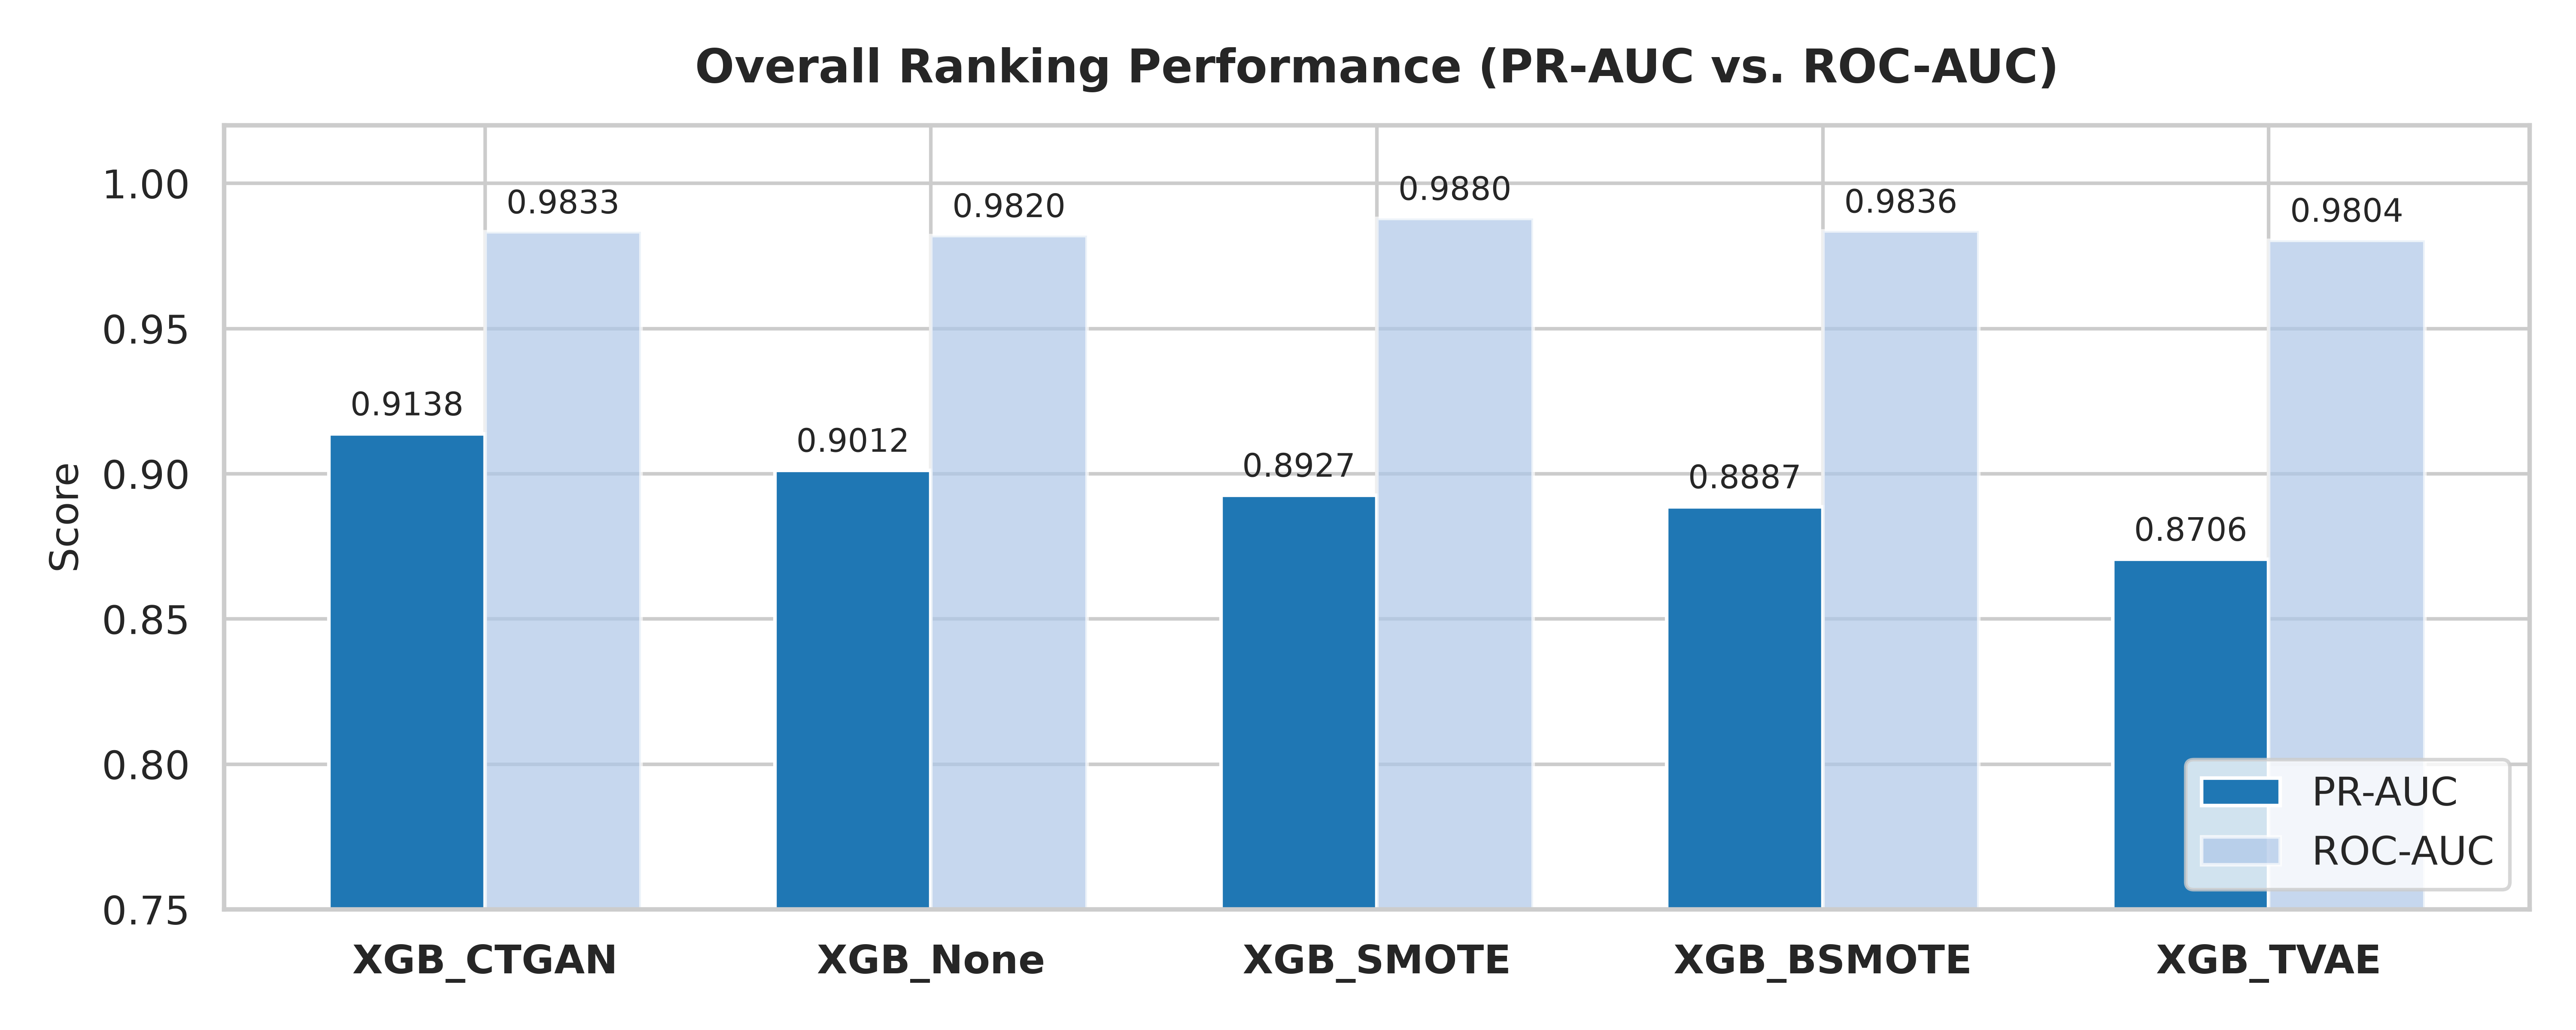
\includegraphics[width=0.80\textwidth]{bar-auc.png}
	\captionsetup{justification=centering}
	\caption{Model-Comparison: Threshold Invariant Metrics.}
	\label{fig:model-perf-thr-inv}
\end{figure}

\begin{figure}[H]
	\centering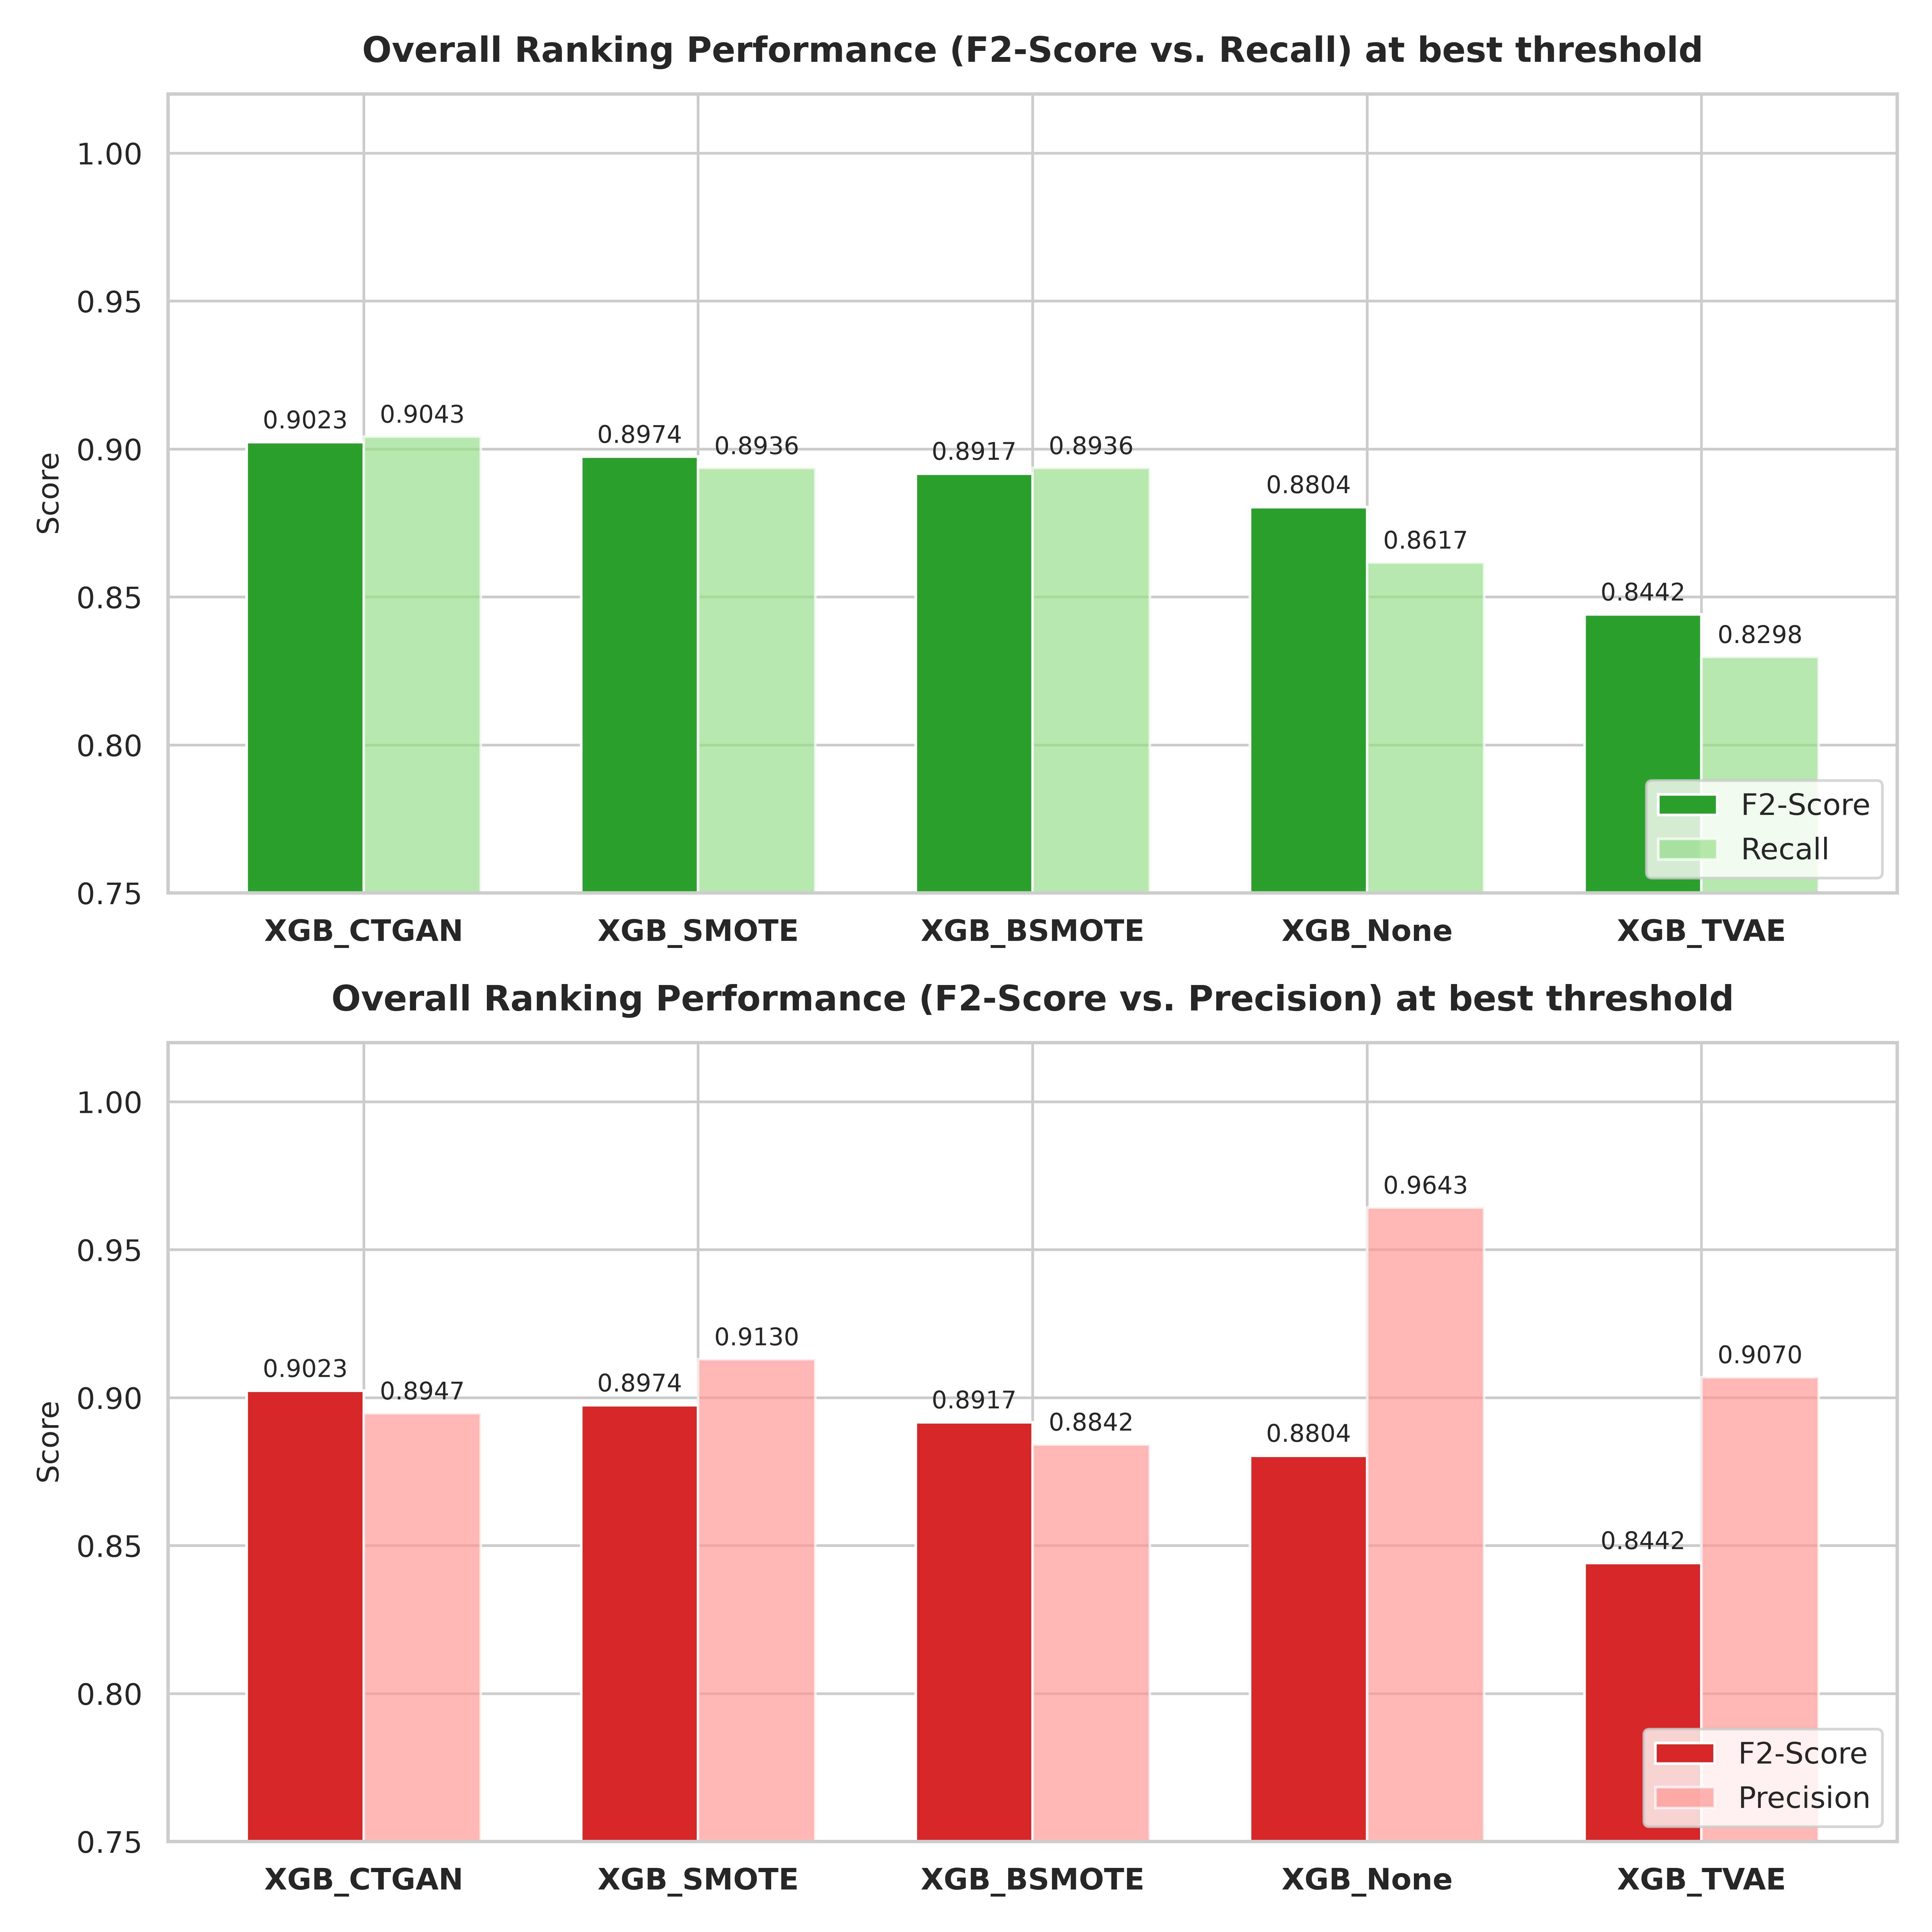
\includegraphics[width=0.75\textwidth]{bar-best-th.png}
	\captionsetup{justification=centering}
	\caption{Model-Comparison: F2-Score, Recall, Precision at model-best threshold.}
	\label{fig:model-best-thr}
\end{figure}


\subsection{Step-2: Generative Model}
We trained both TVAE and CTGAN on full dataset as our generative models to be used in testing and benchmarking our agentic systems. We check them visually using box-plot, feature-by-feature for both minority and majority class which is not easy to conclude (60-plot, each contain 3 box-plot side by side!). Then we used SDMetrics library (Synthetic data evaluation metrics)~\parencite{sdv-git}, which we can be used for numerical evaluation of our generative models, and the result are given in Table~\ref{tab:gen-model-quality-score}.  If we were going to judge based on these results, TVAE will be a winner, because for Fraud-class TVAE is an obvious winner both in term of overall quality score (87.51\% vs 67.27\%) , and number of winning features (24 vs 6), and on Legit class both TVAE/CTGAN has similar overall score of about (91\%) with a little edge for CTGAN on number of winning features (17 vs 13).

\begin{table}[H]
	\centering
	\caption{Numerical Comparison of Generative models: TVAE vs CTGAN}
	\label{tab:gen-model-quality-score}
	\begin{tabular}{l l c c}
		\toprule
		Class Subset & Model & Overall Quality Score & Feature Wins (out of 30) \\
		\midrule
		\textbf{Fraud ($Class = 1$)} & \textbf{TVAE} & \textbf{87.51\%} & \textbf{24 (80\%)} \\
		& CTGAN & 67.27\% & 6 (20\%)\\
		\addlinespace
		\textbf{Legit ($Class = 0$)} & TVAE & 91.16\% & 13 (43.3\%) \\
		& \textbf{CTGAN} & \textbf{91.62\%} & \textbf{17 (56.7\%)} \\
		\bottomrule
	\end{tabular}
\end{table}

However, using  feature by feature , and number of winning features or overall average score , cannot represent a complex relation between features and how they can determine the classification, Therefore, since our ultimate measures and metrics are PR-AUC, F2-Score, Recall, and Precision, we will use our trained  classifier models in step-1, to determine these metric on the sample generated by these models, and the results are shown in Fig.~\ref{fig:gen-clf-pair} (NOTE: label on these plots shows (Generative-Model, Classification-Model) pair, for example CTGAN-XGB\_SMOTE means we use CTGAN as Generative model, and used XGBoost model trained based on SMOTE oversampling). We also added 80\% line on all plots, to be our minimum requirements on all these metrics, and help to narrow down our model-pair selection.

\begin{figure}[H]
	\centering\includegraphics[width=0.8\textwidth]{select_gen_model_clf_model_pair}
	\captionsetup{justification=centering}
	\caption{Comparison of Generative Model, Classification-Model Pairs.}
	\label{fig:gen-clf-pair}
\end{figure}

Base on Fig.~\ref{fig:gen-clf-pair} we can conclude:
\begin{itemize}
	\item Only  CTGAN-XGB\_CTGAN, and TVAE-XGB\_TVAE have ove 80\% in PR-AUC, which narrow down our selection into these two pairs.
	\item Between these two candidate pairs, when we check the Precision,  CTGAN-XGB\_CTGAN completely outperform TVAE-XGB\_TVAE (approximatly 90\% vs 50\%)
	\item Data Generated by TVAE is also perform well with other classifier models, e.g: with XGB\_BSMOTE, (gray-bar) XGB\_CTGAN (red-bar), or even with XGB\_None (orange-bar).  Even better Precision with these classifier than with XGB\_TVAE (brown-bar).
\end{itemize}

\subsection{Step-3: Dual Threshold and Training Dataset for LTM}
While for single threshold optimization we can use specific metrics, like accuracy, recall, etc, and in our case F2-Score, for dual threshold we need to define a cost function and minimize the total cost. With the same idea to punish FN twice as FP, and \textbf{\textit{extreme simplification, to show the idea}},  we define our cost function as follow:
\begin{itemize}
\item cost of FN: 10.0
\item cost of FP: 5.0
\item cost of using LLM-Agent: 0.2
\item LLM-Agent accuracy: 90\%
\item Note: For simplicity we assume recall and precision accuracy for LLM-agent are the same.
\end{itemize}

Optimization contour-plot for generated-data shown in Fig.~\ref{fig:dual-threshold-opt-gen} (for real-data, please see the notebook), The effect of dual-threshold which keep FP/FN at  the minimum values between single thresholds show in the confusion matrix in Fig.~\ref{fig:dual-threshold-opt-effect} 


\begin{figure}[H]
\centering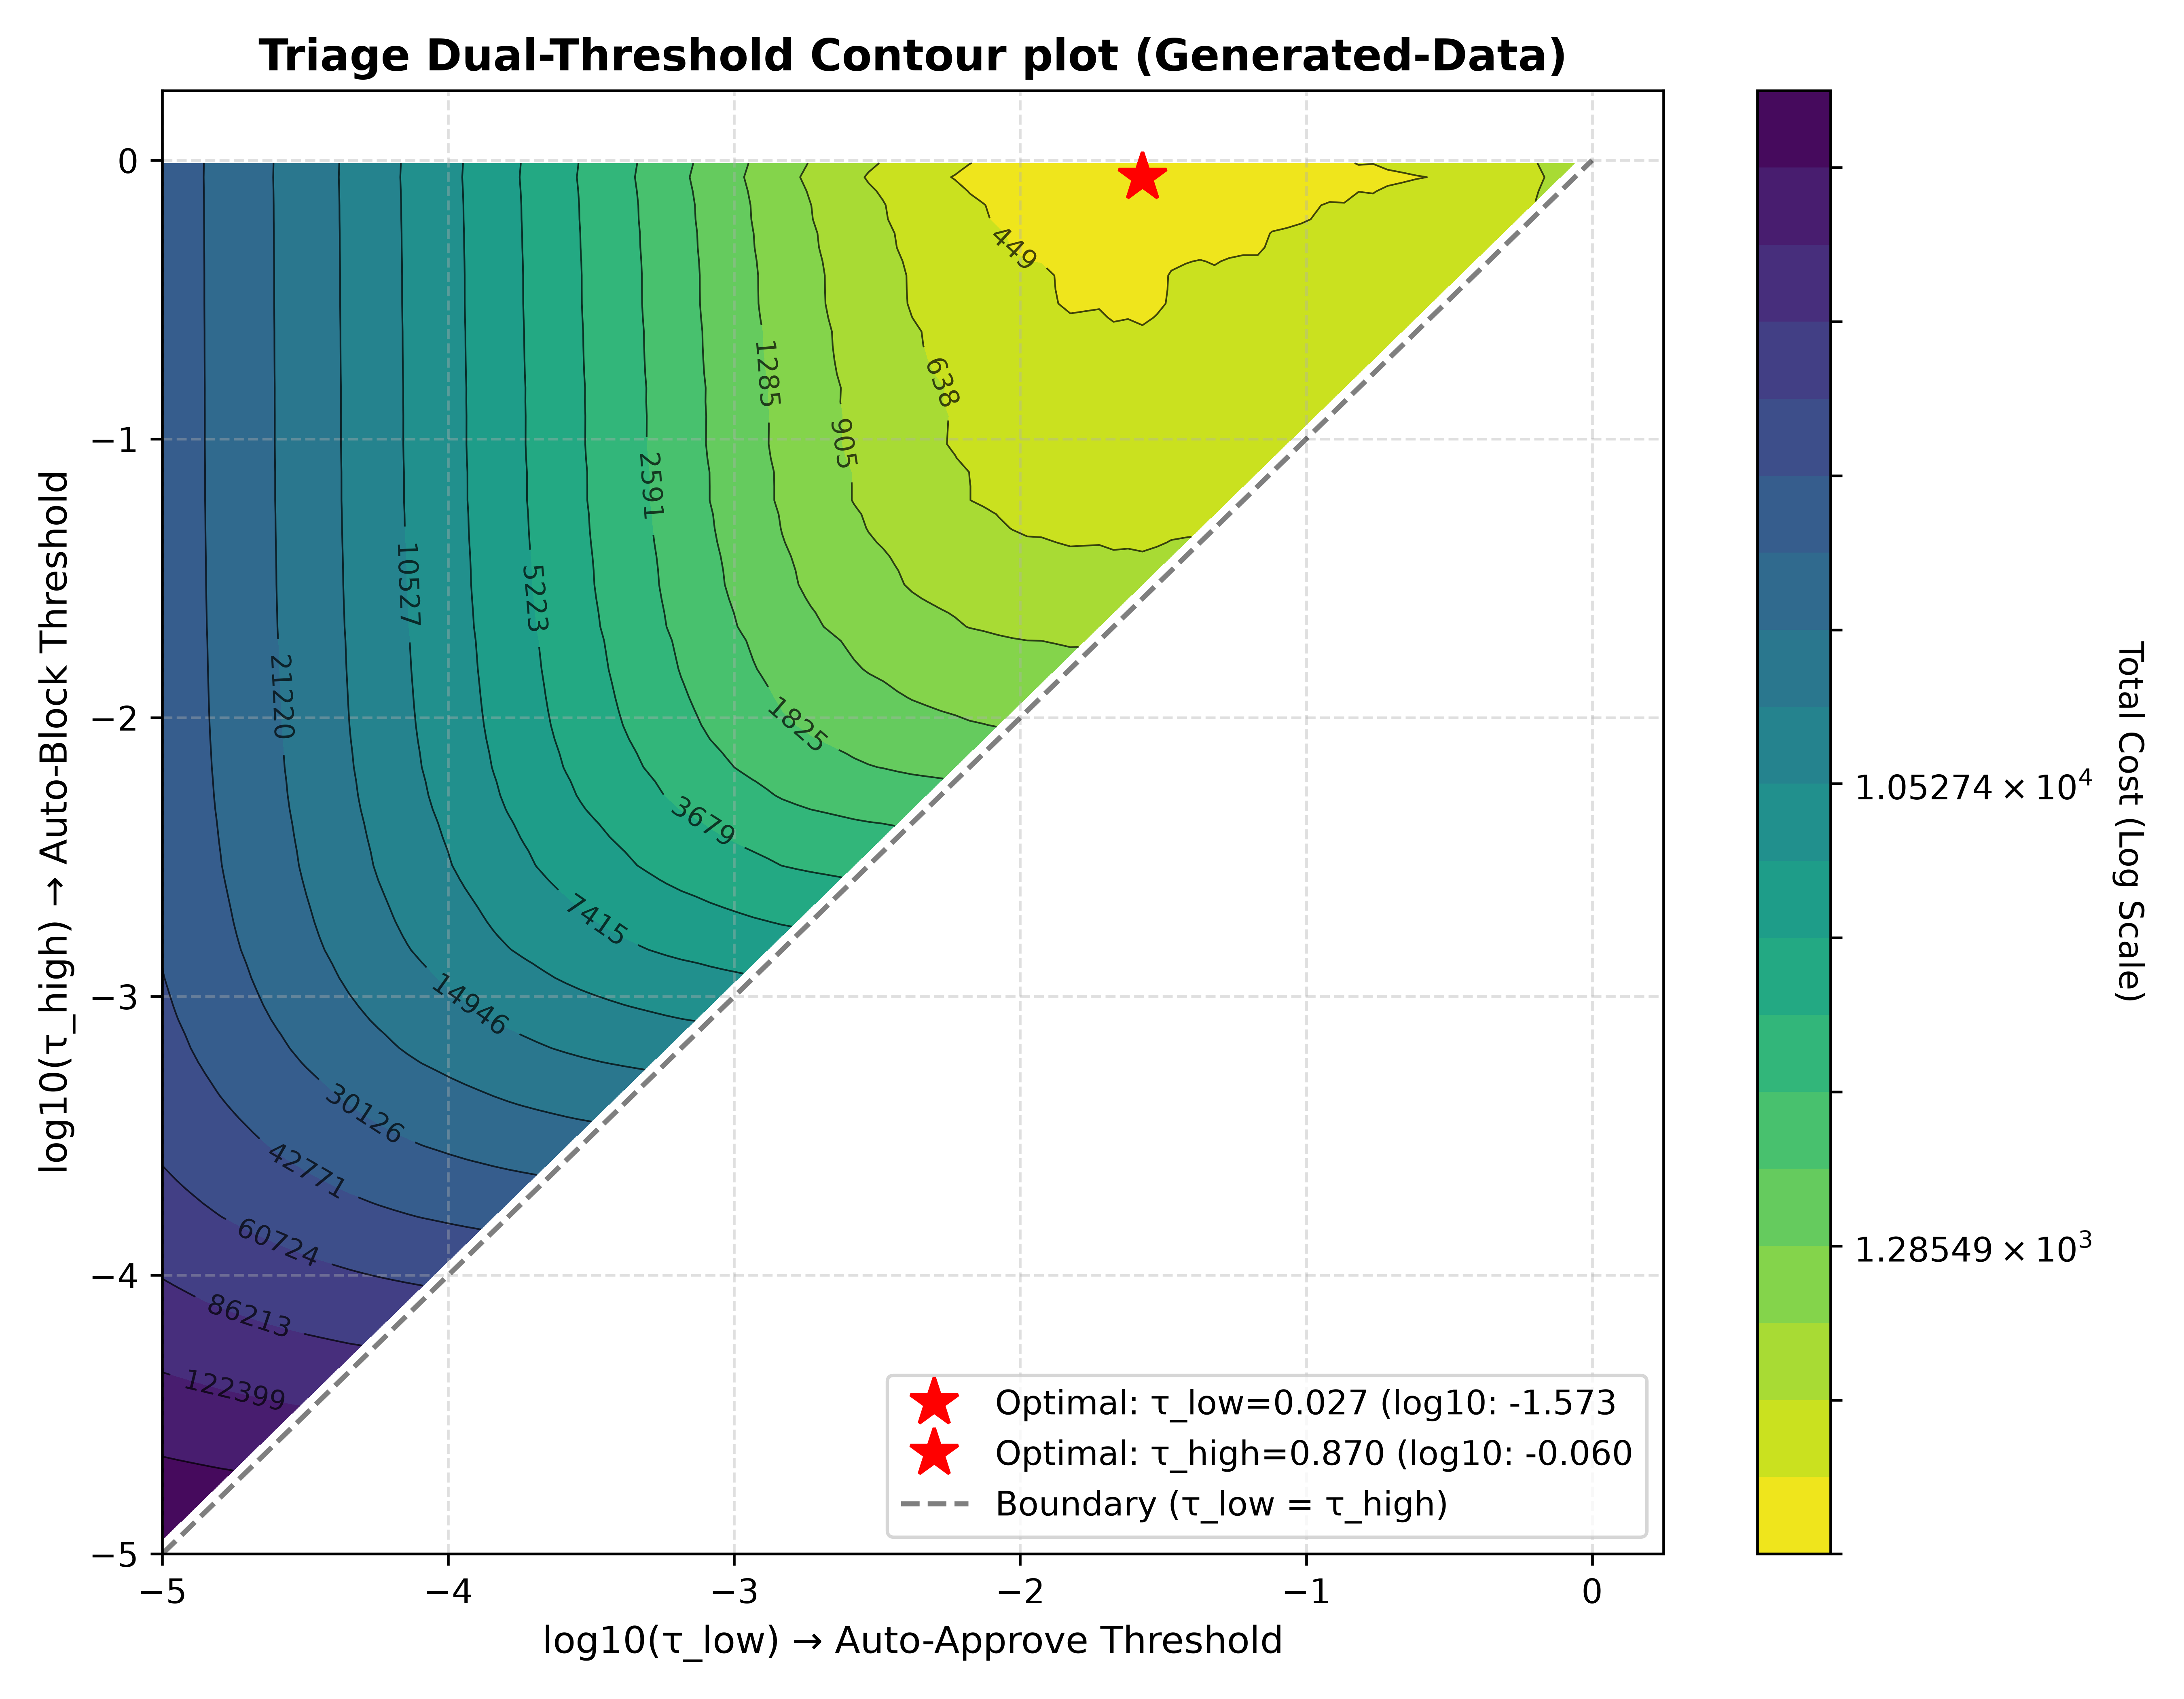
\includegraphics[width=0.95\textwidth]{dual_thr_opt_gen_data}
\captionsetup{justification=centering}
\caption{Dual Threshold Optimization, Contour Plot for Generated Data.}
\label{fig:dual-threshold-opt-gen}
\end{figure}

\begin{figure}[H]
\centering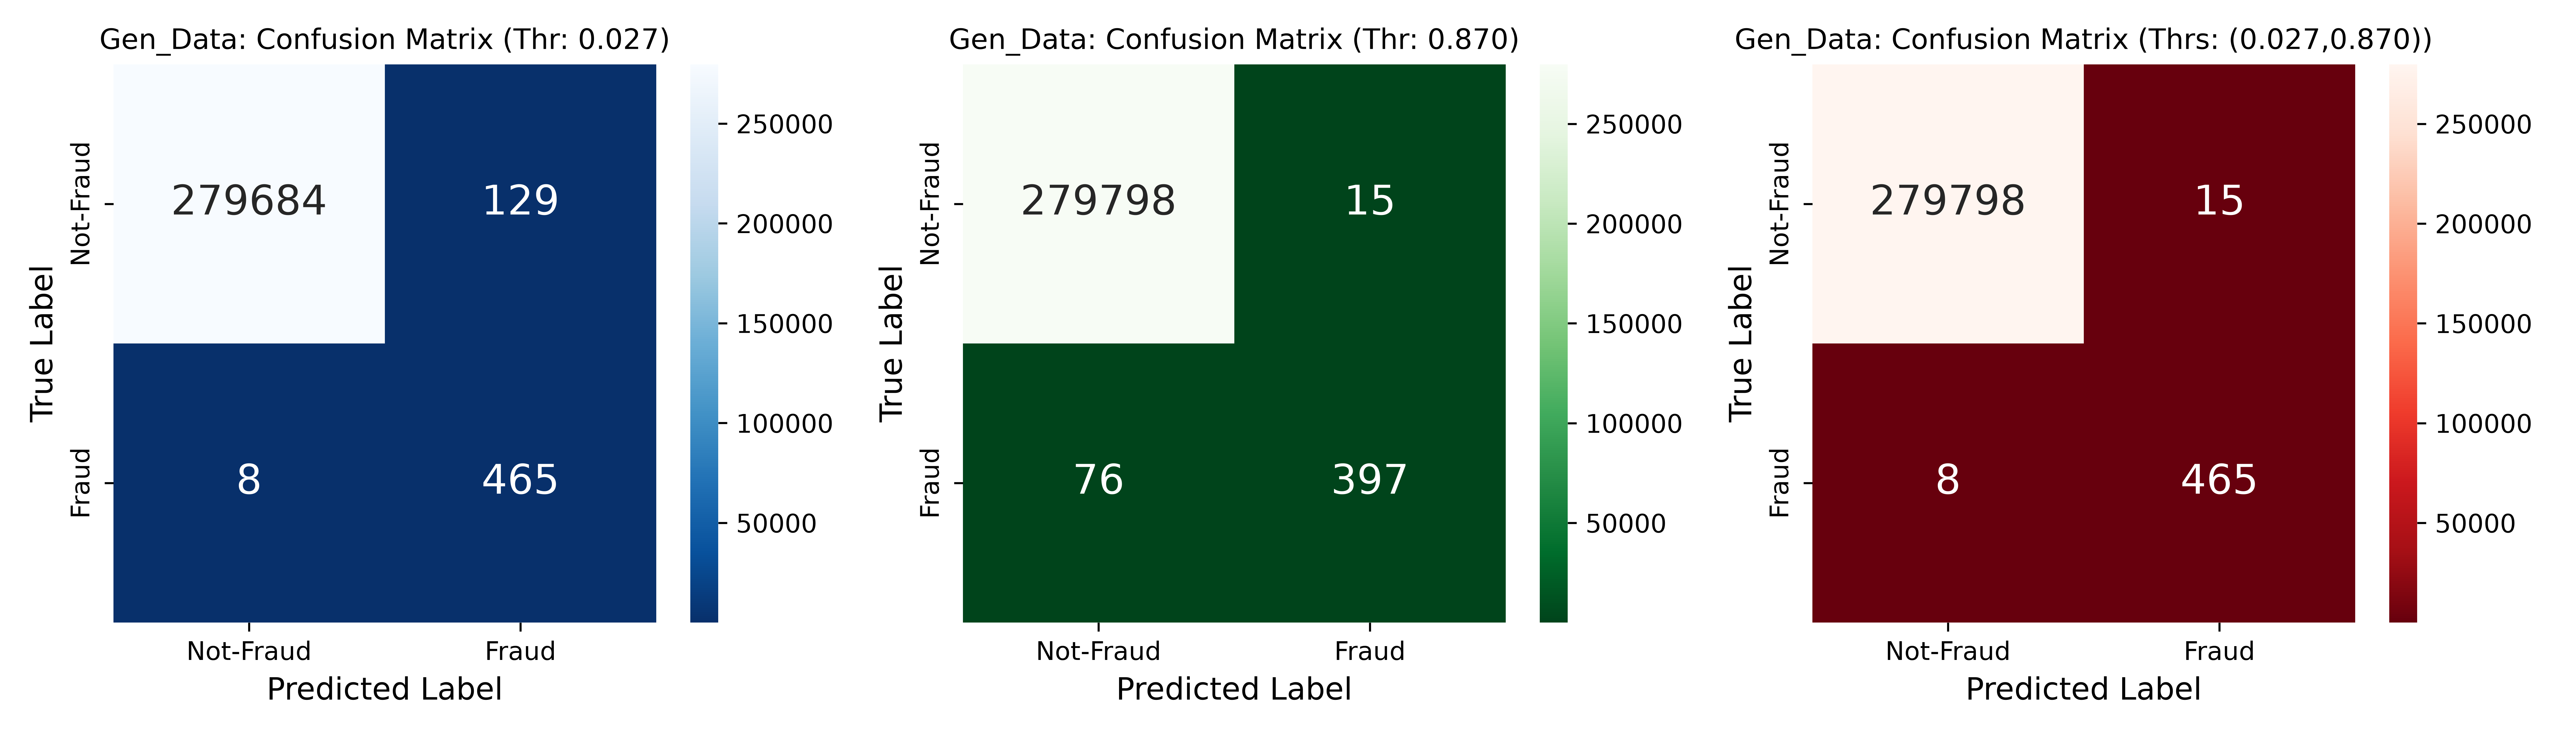
\includegraphics[width=1.0\textwidth]{dual_thr_conf_mat_gen_data}
\captionsetup{justification=centering}
\caption{Dual Threshold Optimization Effect on Minimizing FP/FN.}
\label{fig:dual-threshold-opt-effect}
\end{figure}

For example Dual-Threshold-FP = min(129, 15), As we can see in Fig.~\ref{fig:dual-threshold-opt-effect}.

With applying the optimized dual thresholds on real or generated data we can prepare samples to initialize our Long-Term Memory (Vector-database) to be used by LLM-Agent.

\section{Ethical Considerations and Responsible AI}
Automated financial screening introduces important ethical dimensions regarding fairness, transparency, and accountability:
\begin{itemize}
	\item \textbf{Algorithmic Bias \& False Positives:} Imbalanced datasets risk generating biased rules that unfairly target specific demographic spending behaviors as anomalous.
	\item \textbf{Human-in-the-Loop Accountability:} By incorporating mandatory human escalation for low-confidence decisions, the system prevents autonomous wrongful account blocking and ensures user due process.
	\item \textbf{Data Privacy:} Synthetic data generation (CTGAN) helps mitigate privacy leakage by supplementing training pipelines without over-relying on sensitive real-world cardholder records.
\end{itemize}

\section{Evaluation and Reflection}

Sample agentic-system run  without escalation (Fig.~\ref{fig:no-escalate}), escalate to LLM (Fig.~\ref{fig:escalate2llm}), and escalate up to Human (Fig.~\ref{fig:escalate2human}) are shown below. (For all possible scenarios including when Agent make mistake and create FP see the \verb|step4_agentic_test_results| notebook or its html version)

\begin{figure}[H]
	\centering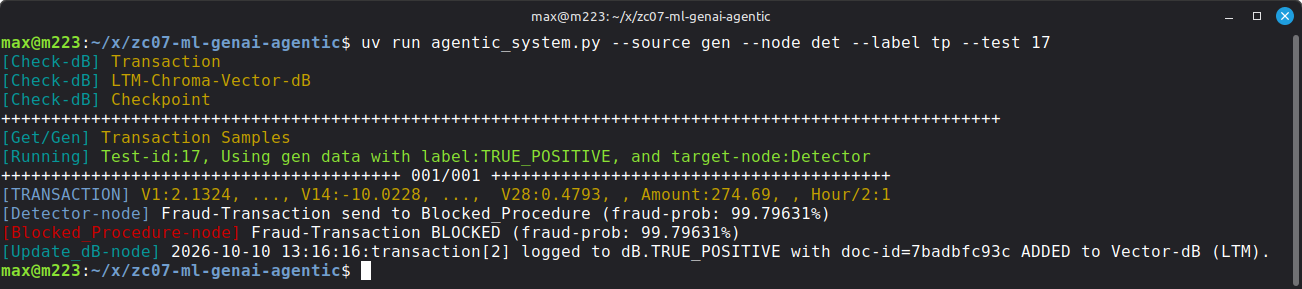
\includegraphics[width=0.9\textwidth]{z-det-tp}
	\captionsetup{justification=centering}
	\caption{Sample Agentic Workflow Without Escalation.}
	\label{fig:no-escalate}
\end{figure}

\begin{figure}[H]
	\centering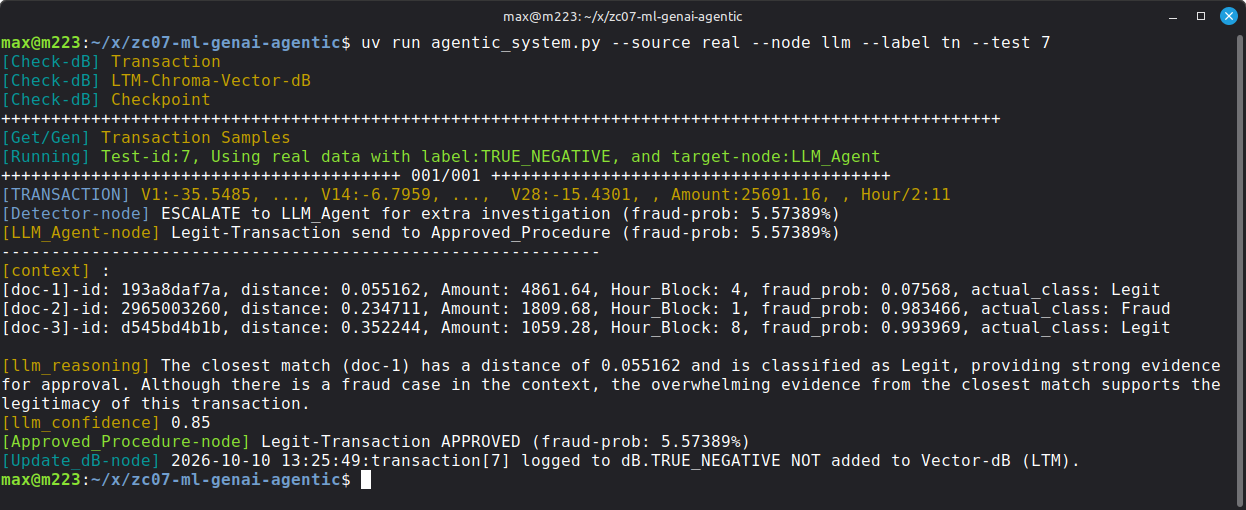
\includegraphics[width=0.9\textwidth]{z-llm-real-tn-07}
	\captionsetup{justification=centering}
	\caption{Sample Agentic Workflow Escalated to LLM.}
	\label{fig:escalate2llm}
\end{figure}


\begin{figure}[H]
	\centering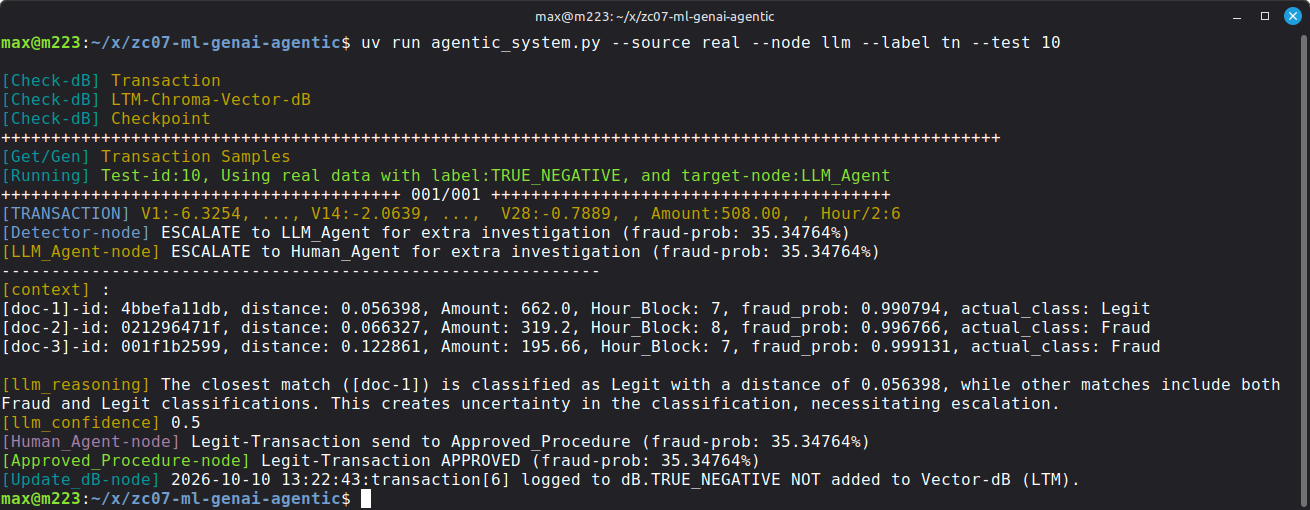
\includegraphics[width=0.9\textwidth]{z-llm-real-tn-10}
	\captionsetup{justification=centering}
	\caption{Sample Agentic Workflow Escalated to Human.}
	\label{fig:escalate2human}
\end{figure}

When we prepared data for LTM, in step-3, we split them 50\%-50\% into training and testing dataset, we will use training dataset for initializing LTM, and testing (test-cases) for our test. In total we have 661 test-cases which is a mixture of data from real-dataset, and generated(gen)-dataset, and targeting our Detector-Node (Dual-Threshold Classifier) or LLM-Agent Node as shown in Table~\ref{tab:test}

	\begin{table}[!h]
	\centering
	\caption{Test-cases Information.}
	\label{tab:test}
	\begin{tabular}{lrrrrr}
		\toprule
		& TP & TN & FN & FP & Row\_Count \\
		node\_source &  &  &  &  &  \\
		\midrule
		Detector-real & 225 & 50 & 4 & 2 & 281 \\
		LLM\_Agent-real & 8 & 21 & 0 & 0 & 29 \\
		Detector-gen & 199 & 50 & 4 & 7 & 260 \\
		LLM\_Agent-gen & 34 & 57 & 0 & 0 & 91 \\
		Column\_Sum & 466 & 178 & 8 & 9 & \textbf{661} \\
		\bottomrule
	\end{tabular}
\end{table}		


For detector-node we have FP/FN, because these FP/FN are the results of our ML classifier, and we cannot get rid of them unless we could train a better classifier models. For LLM node, there is no FP or FN sample in the above table, FP or FN will be created depends on LLM-Agent decision which in turn also depends on how good is the content of  LTM, and we will see the result after test.

While real-dataset is limited, we can increase test-cases using generated data, as far as we have budget to spend for LLM cost! Therefore to limit our cost, we use limited number of generated data, too.

The first time we run all test cases, LLM  has only the LTM initialized with (training cases), but if we run the test-cases again, we expect that LLM to have perfect decision, because LTM should have all the previous mistake. The  confusion-matrix of the results shown in Fig.~\ref{fig:final-conf-mat}, and corresponding numerical metrics collected in Table~\ref{tab:final-metric}.

\begin{figure}[H]
	\centering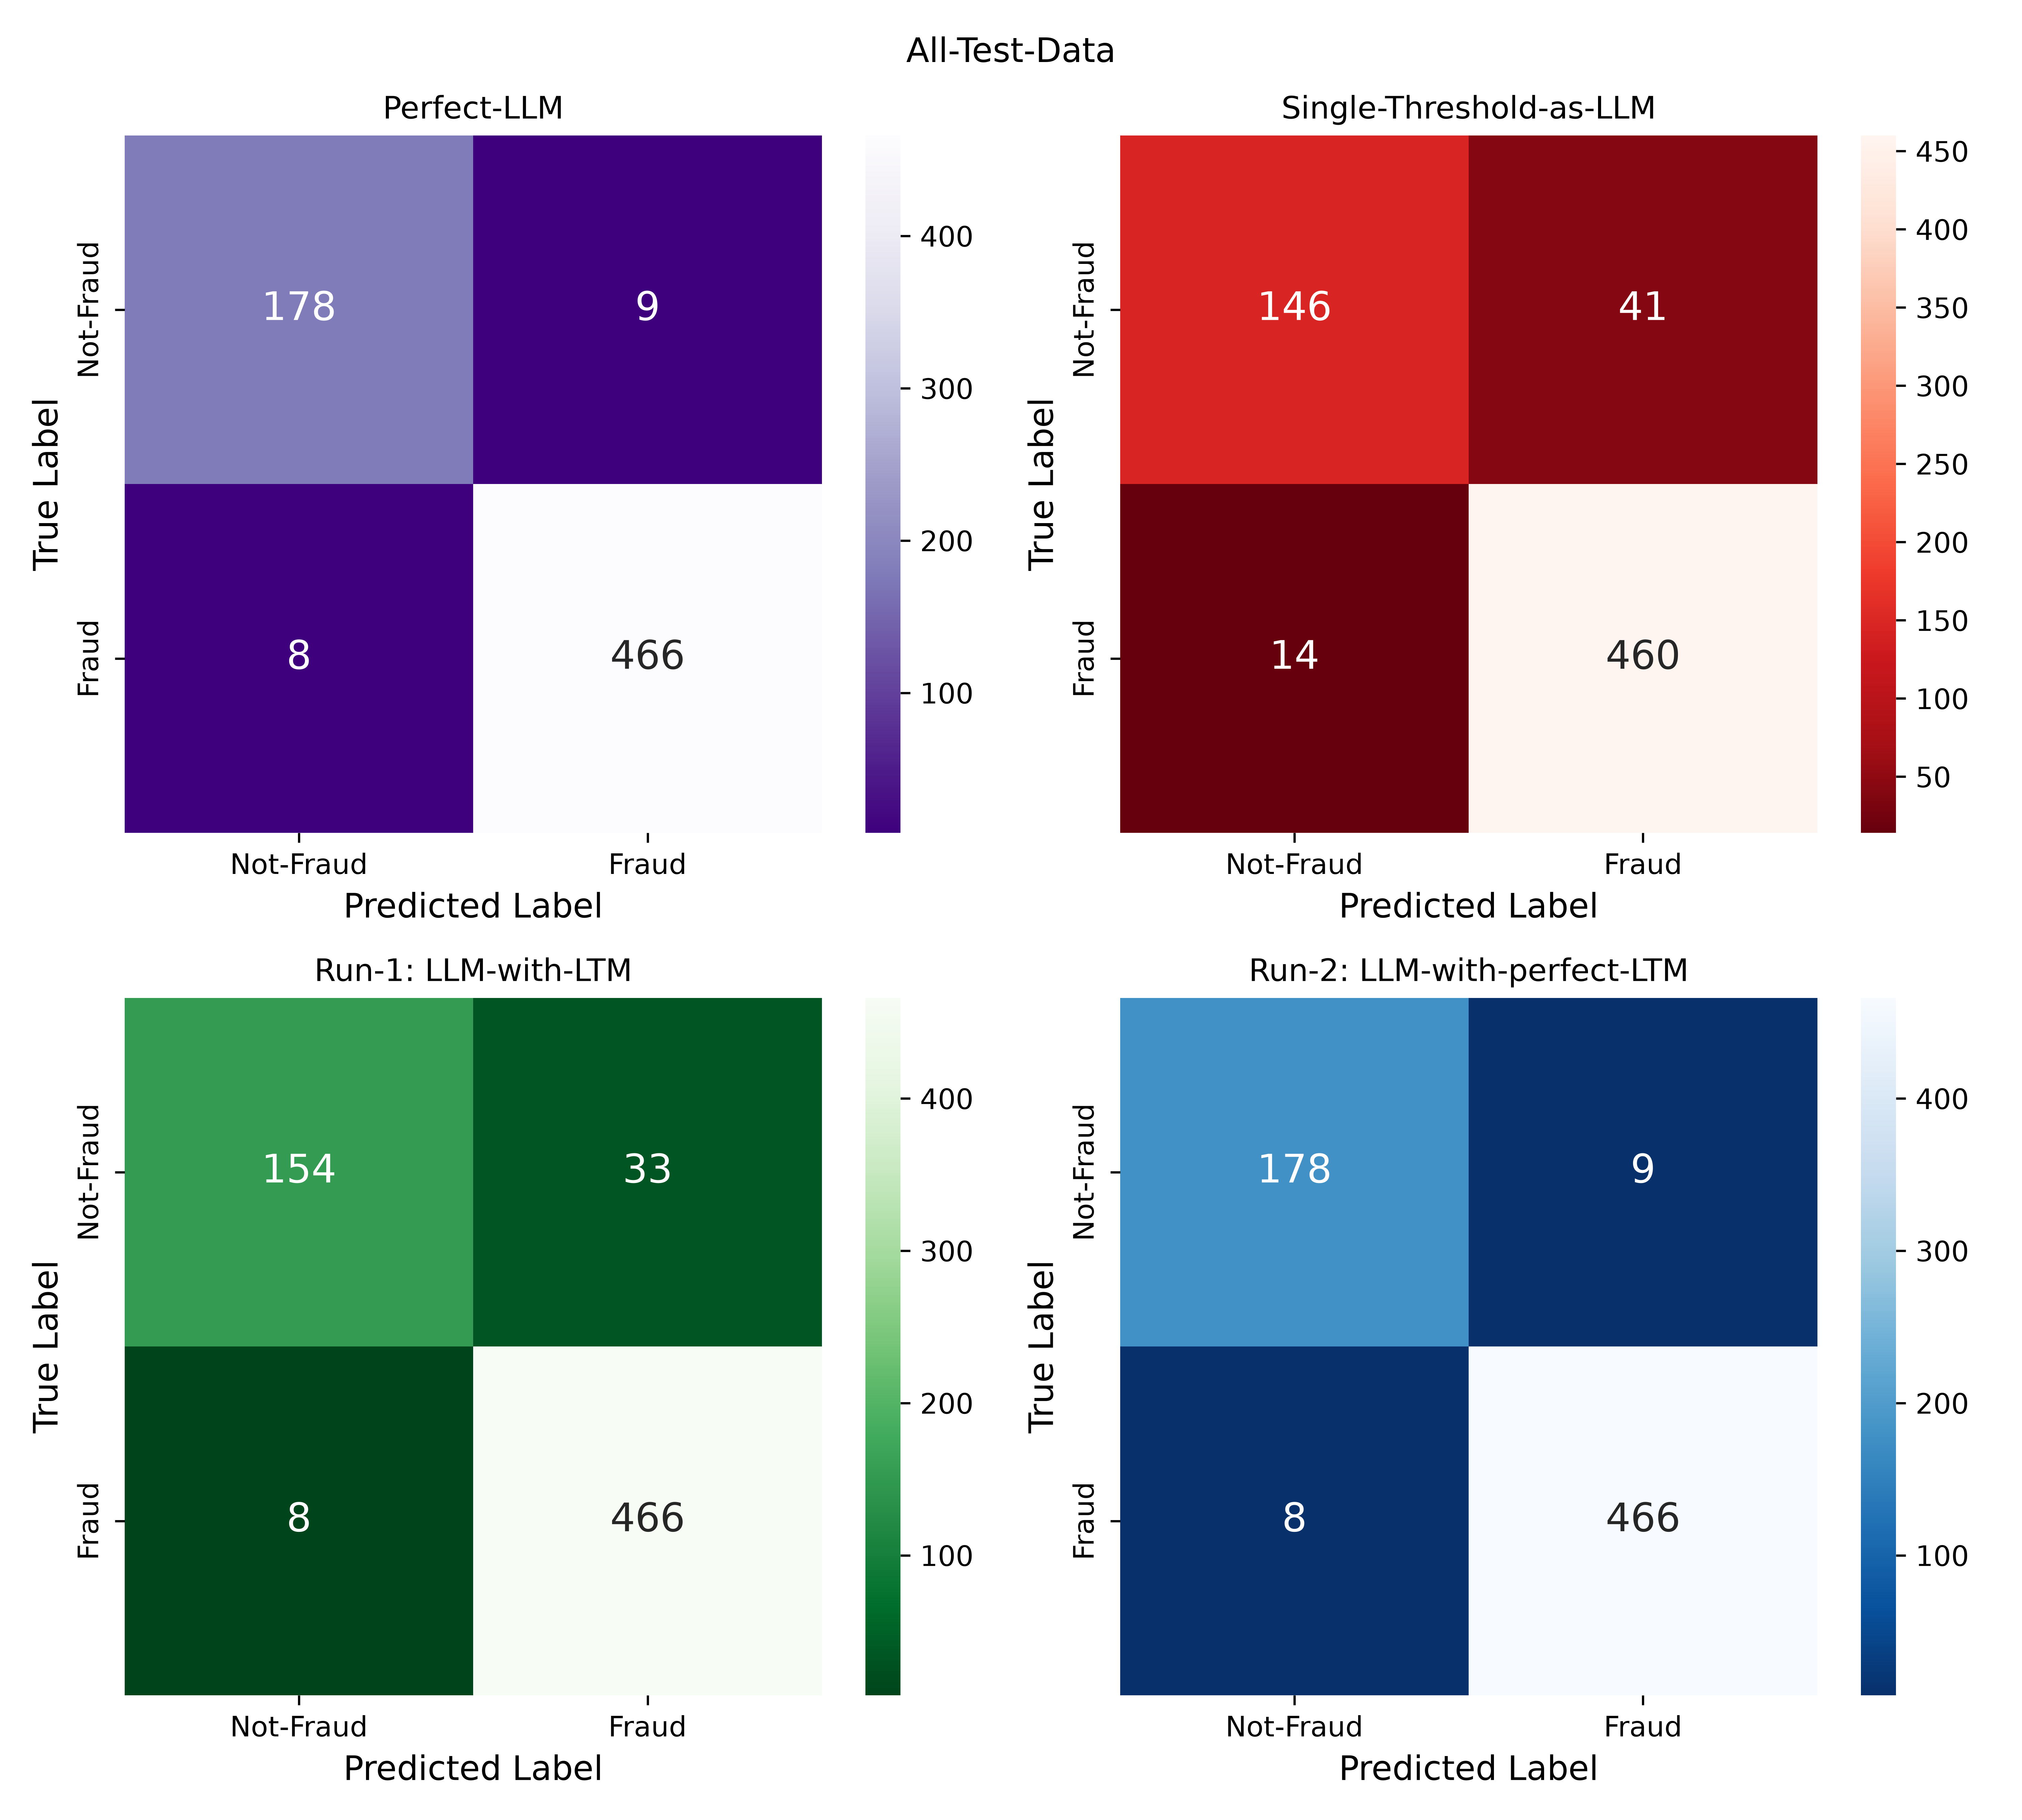
\includegraphics[width=0.9\textwidth]{conf_mat_all_test_data_cmp.png}
	\captionsetup{justification=centering}
	\caption{Confusion Matrix for All Test-Case Run.}
	\label{fig:final-conf-mat}
\end{figure}

\begin{table}[H]
	\centering
	\caption{Metrics for All Test-Case Run.}
	\label{tab:final-metric}
	\begin{tabular}{lrrrrr}
		\toprule
		Run-Info& Accuracy & Precision & Recall & F1-Score & F2-Score \\	
		\midrule
		Perfect-LLM & 97.43 & 98.11 & 98.31 & 98.21 & 98.27 \\
		Single-Threshold-as-LLM & 91.68 & 91.82 & 97.05 & 94.36 & 95.95 \\
		Run-1: LLM-with-LTM & 93.80 & 93.39 & 98.31 & 95.79 & 97.29 \\
		Run-2: LLM-with-perfect-LTM & 97.43 & 98.11 & 98.31 & 98.21 & 98.27 \\
		\bottomrule
	\end{tabular}
\end{table}

Comparison between \textbf{Single-Threshold-as-LLM}  and  \textbf{Run-1: LLM-with-LTM} shows that how using LLM with initialized LTM, avoid adding any FN (beyond what happened at detector node which is the accuracy of our Classification-Model), but single -threshold actually adds up 6 more FN, and for FP, while LLM agent add extra 24 FP, but with more mature LTM they can be reduced (as we see in Run-2 as ideal LTM), but single threshold agent add extra 32 FP, which results in 1.34\% reduction in F2-Score (97.29\% to 95.95\%)

Based on the above result (Run-1), we can calculate agent-metrics as : 

\begin{multicols}{4}
\begin{itemize}
	\item \textbf{Accuracy} 80.00\%
	\item \textbf{Precision} 63.64\%
	\item \textbf{Recall}  100.00\%	
	\item \textbf{F2-Score} 89.74\%
\end{itemize}
\end{multicols}


This shows that Agent really avoid FN since in the prompt we emphasize that.  Also it shows that the recall/precision for agent is not the same, and after more test, we may need to update our cost function, and define different recall/precision values instead of single accuracy for agent and re-calculate the optimal dual threshold which we consider it as future work after more more tests in real production environment.

Rigorous testing across 661 cases demonstrated strong performance ($F_2$-Score of 97.29\% with LTM). Key takeaways include:
\begin{itemize}
	\item \textbf{Successes:} Dual thresholds successfully filtered unambiguous traffic, allowing the LLM and human agents to focus solely on high-risk edge cases. Long-Term Memory (LTM) integration markedly improved sequential accuracy.
	\item \textbf{Limitations:} Initial agent prompt engineering caused asymmetric precision/recall behavior compared to assumptions in the cost function, highlighting the need to decouple agent-specific precision and recall metrics during optimization.
	\item  \textbf{Potential Metric Inflation}: Due to limited fraud samples (only 473), the same data (or portions of it) was leveraged in both step-1, and step-2.  This approach was necessary for initial feasibility, it can introduces \textit{data leakage}, potentially leading to optimistic metrics.  Let say, we have 5\% performance inflation, then the realistic F2-Score is  92.2\%.  Solution for production discussed in last section.
\end{itemize}

\subsection{Agentic System Analytics}
We also use LangGraph Checkpoint database to  plot our agentic workflow analytics shown in Fig.~\ref{fig:analytics}

\begin{figure}[H]
	\centering
	% Top-left subplot
	\begin{subfigure}[b]{0.48\textwidth}
		\centering
		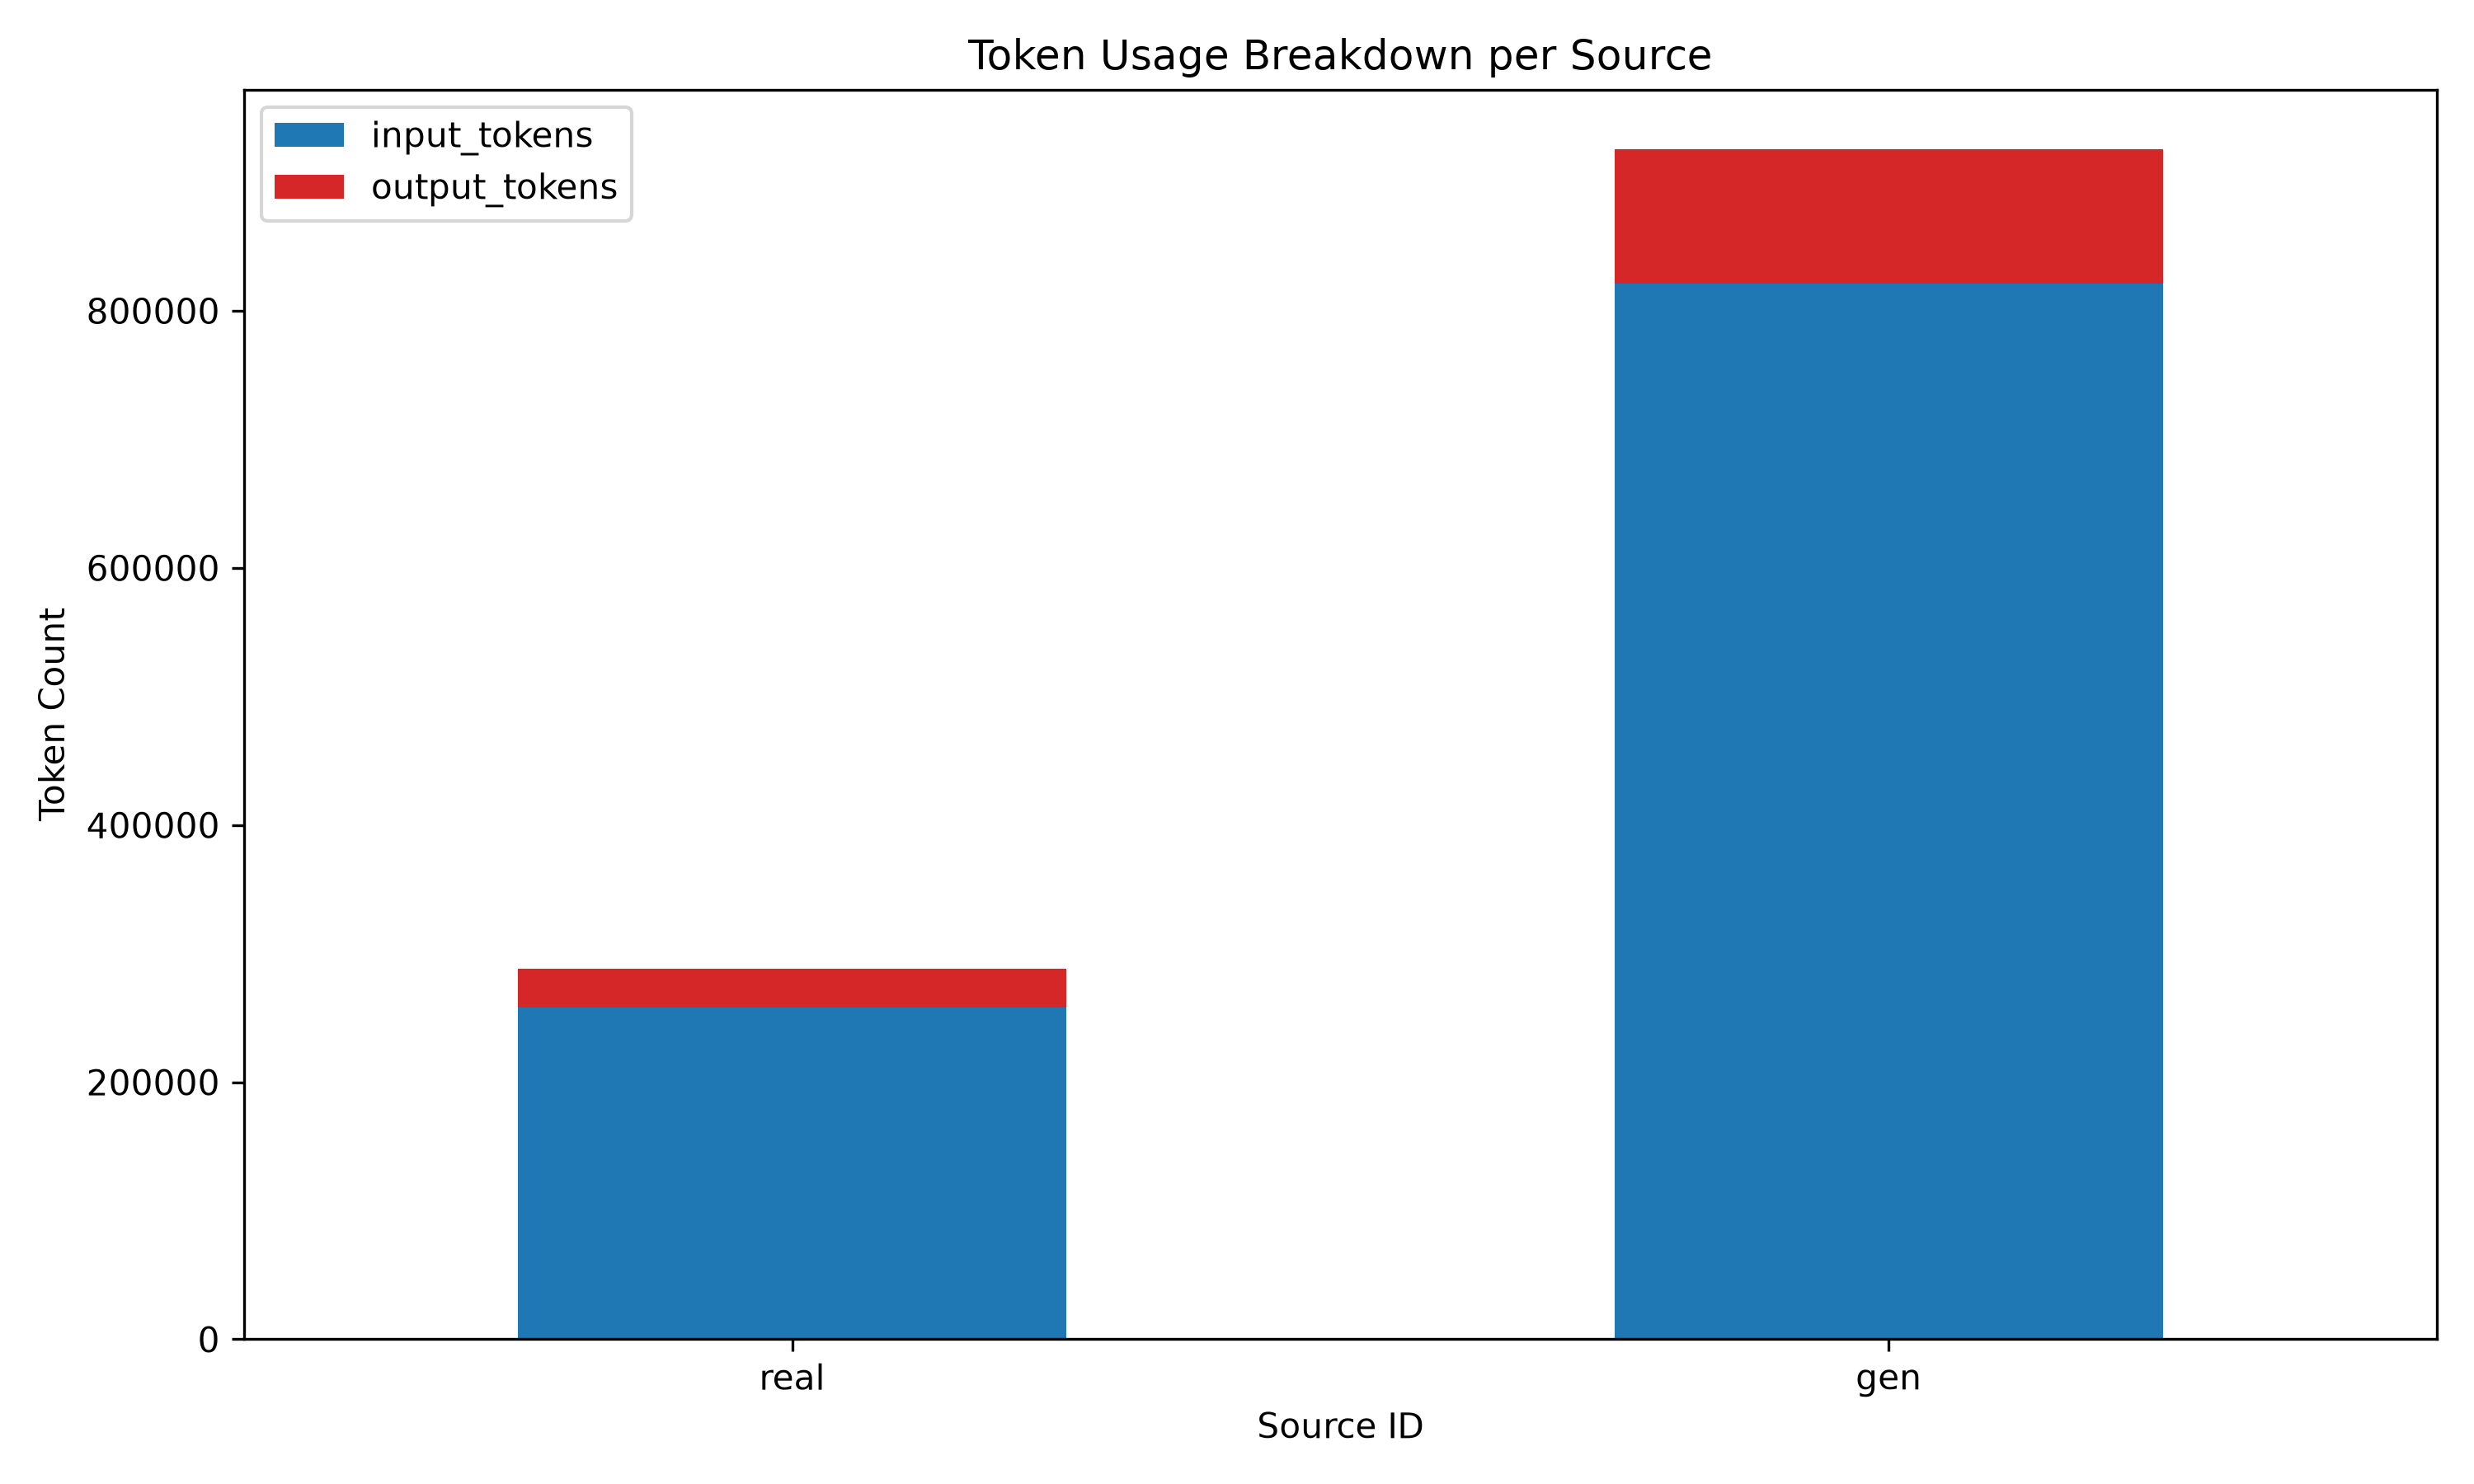
\includegraphics[width=\textwidth]{token_usage}
		%\caption{First Plot ($\sin(x)$)}
		\label{fig:plot1}
	\end{subfigure}
	\hfill
	% Top-right subplot
	\begin{subfigure}[b]{0.48\textwidth}
		\centering
		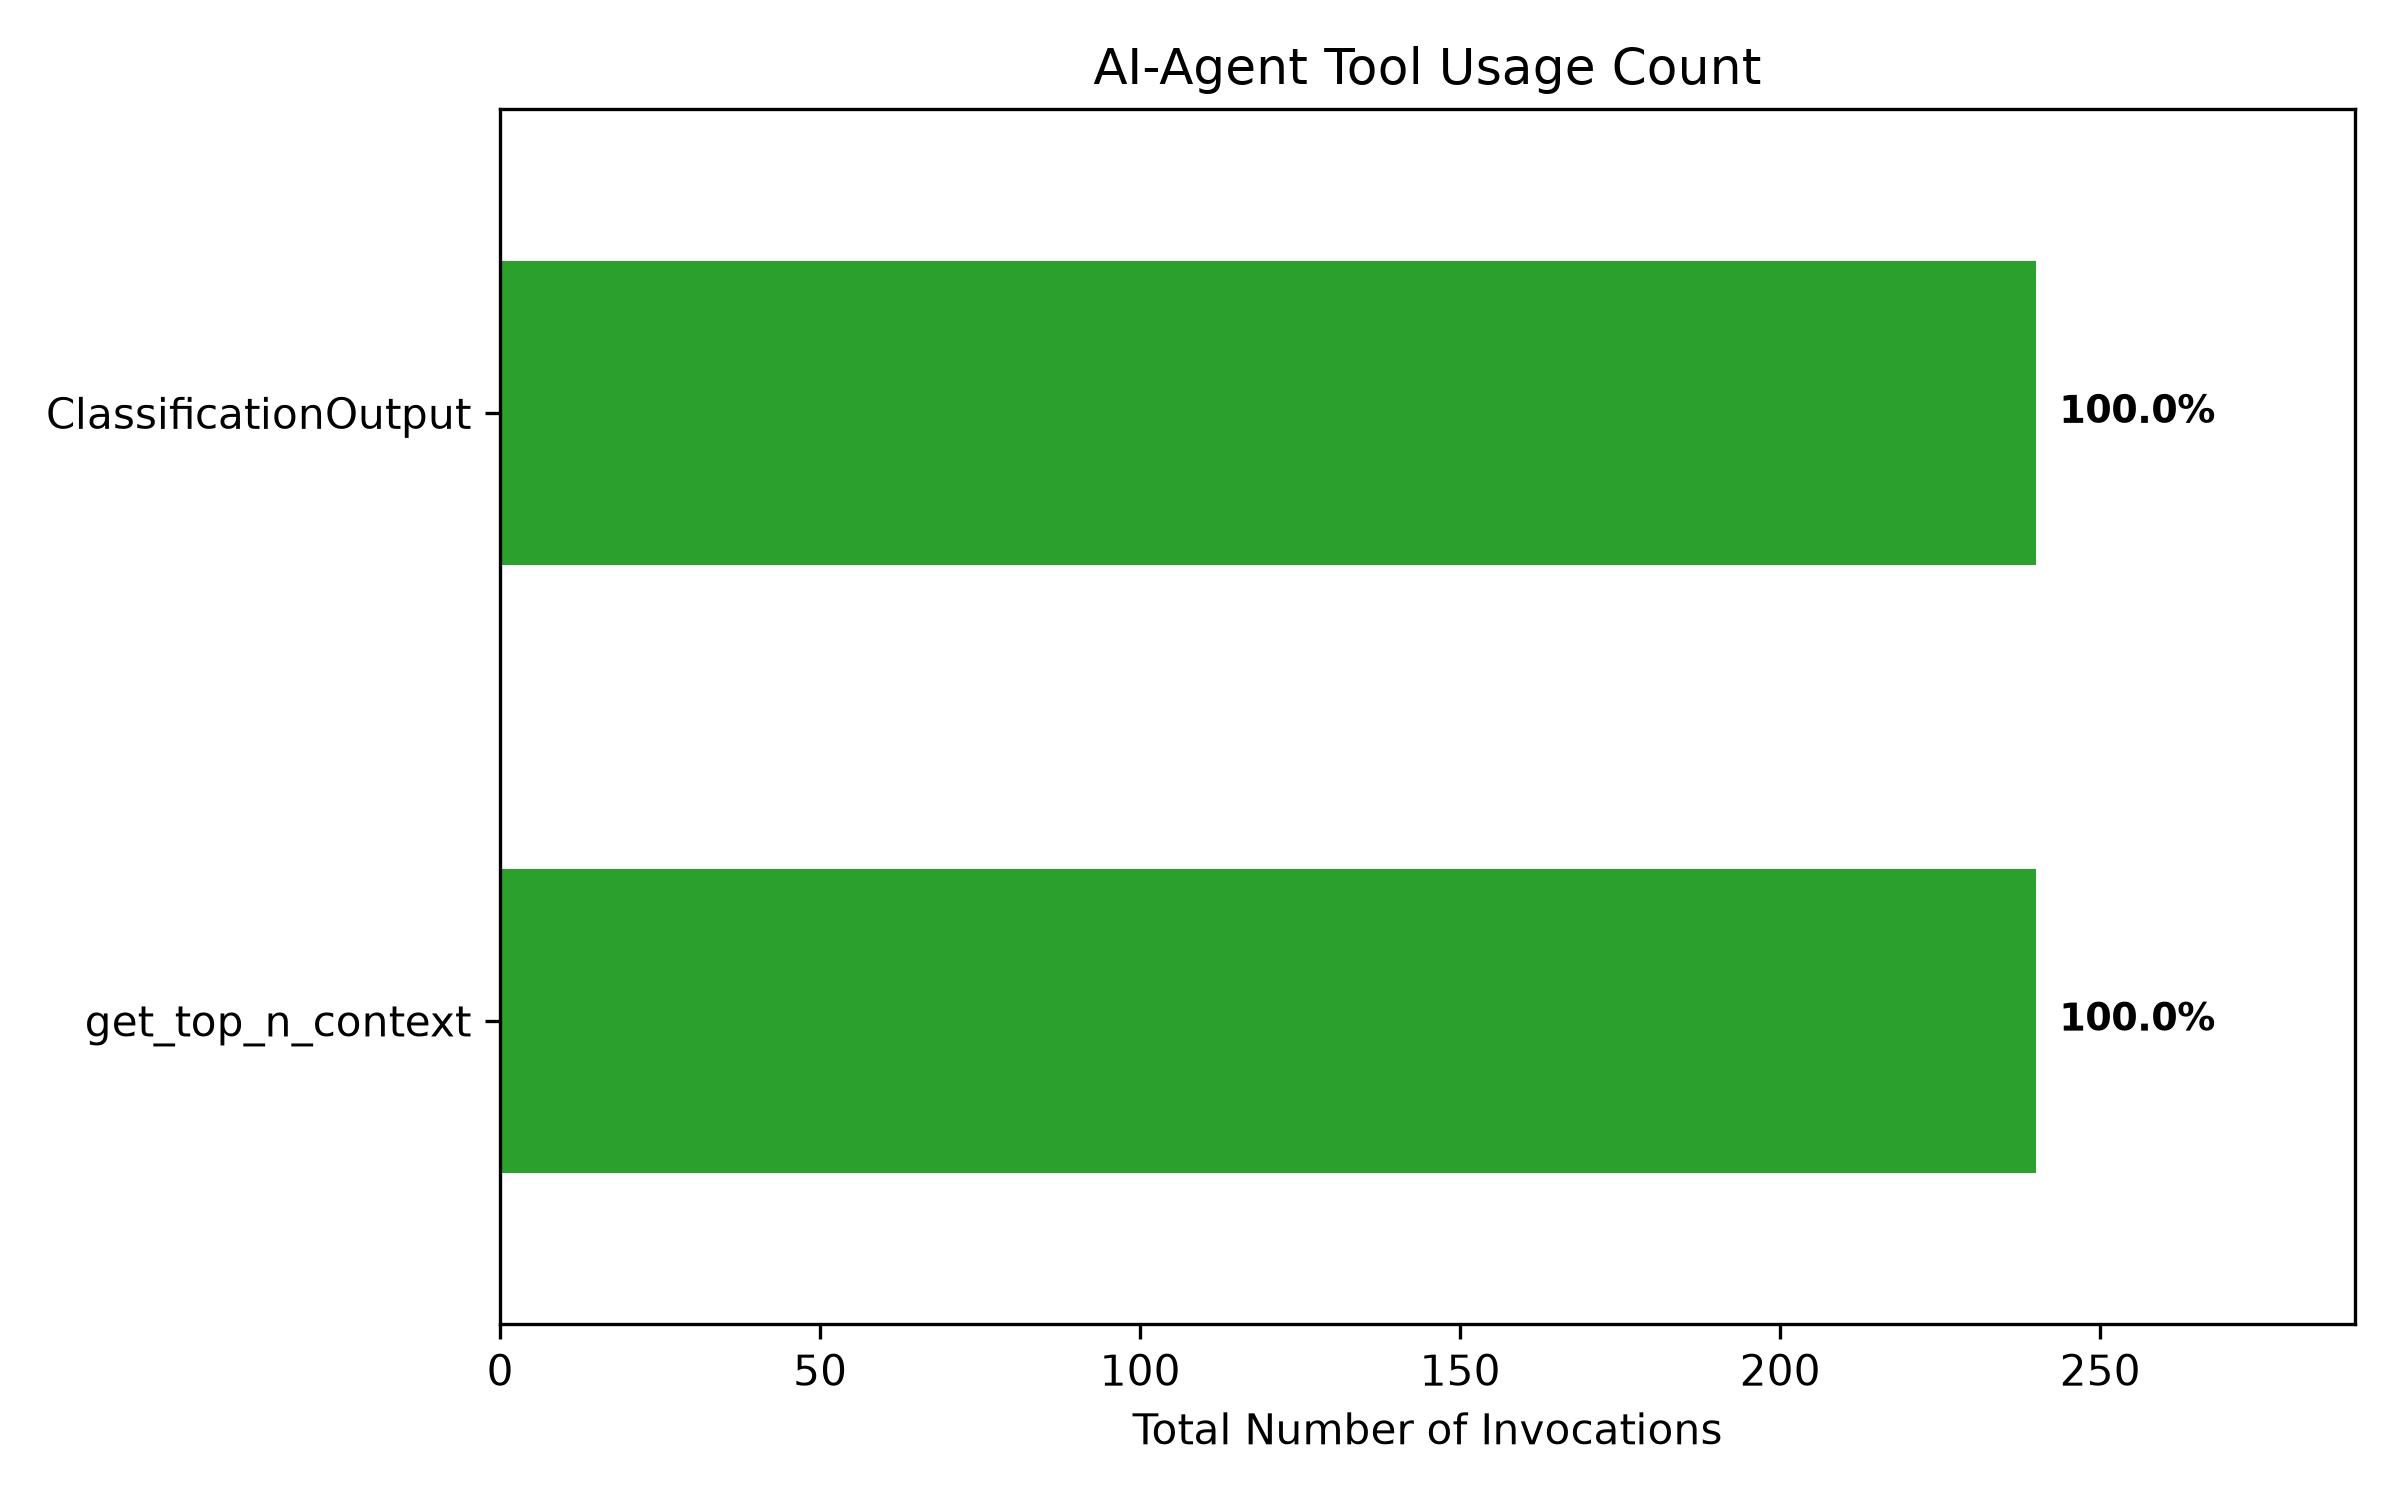
\includegraphics[width=\textwidth]{tool_usage.png}
		%\caption{Second Plot ($\cos(x)$)}
		\label{fig:plot2}
	\end{subfigure}
	
	\vspace{1em}
	
	% Bottom-left subplot
	\begin{subfigure}[b]{0.48\textwidth}
		\centering
		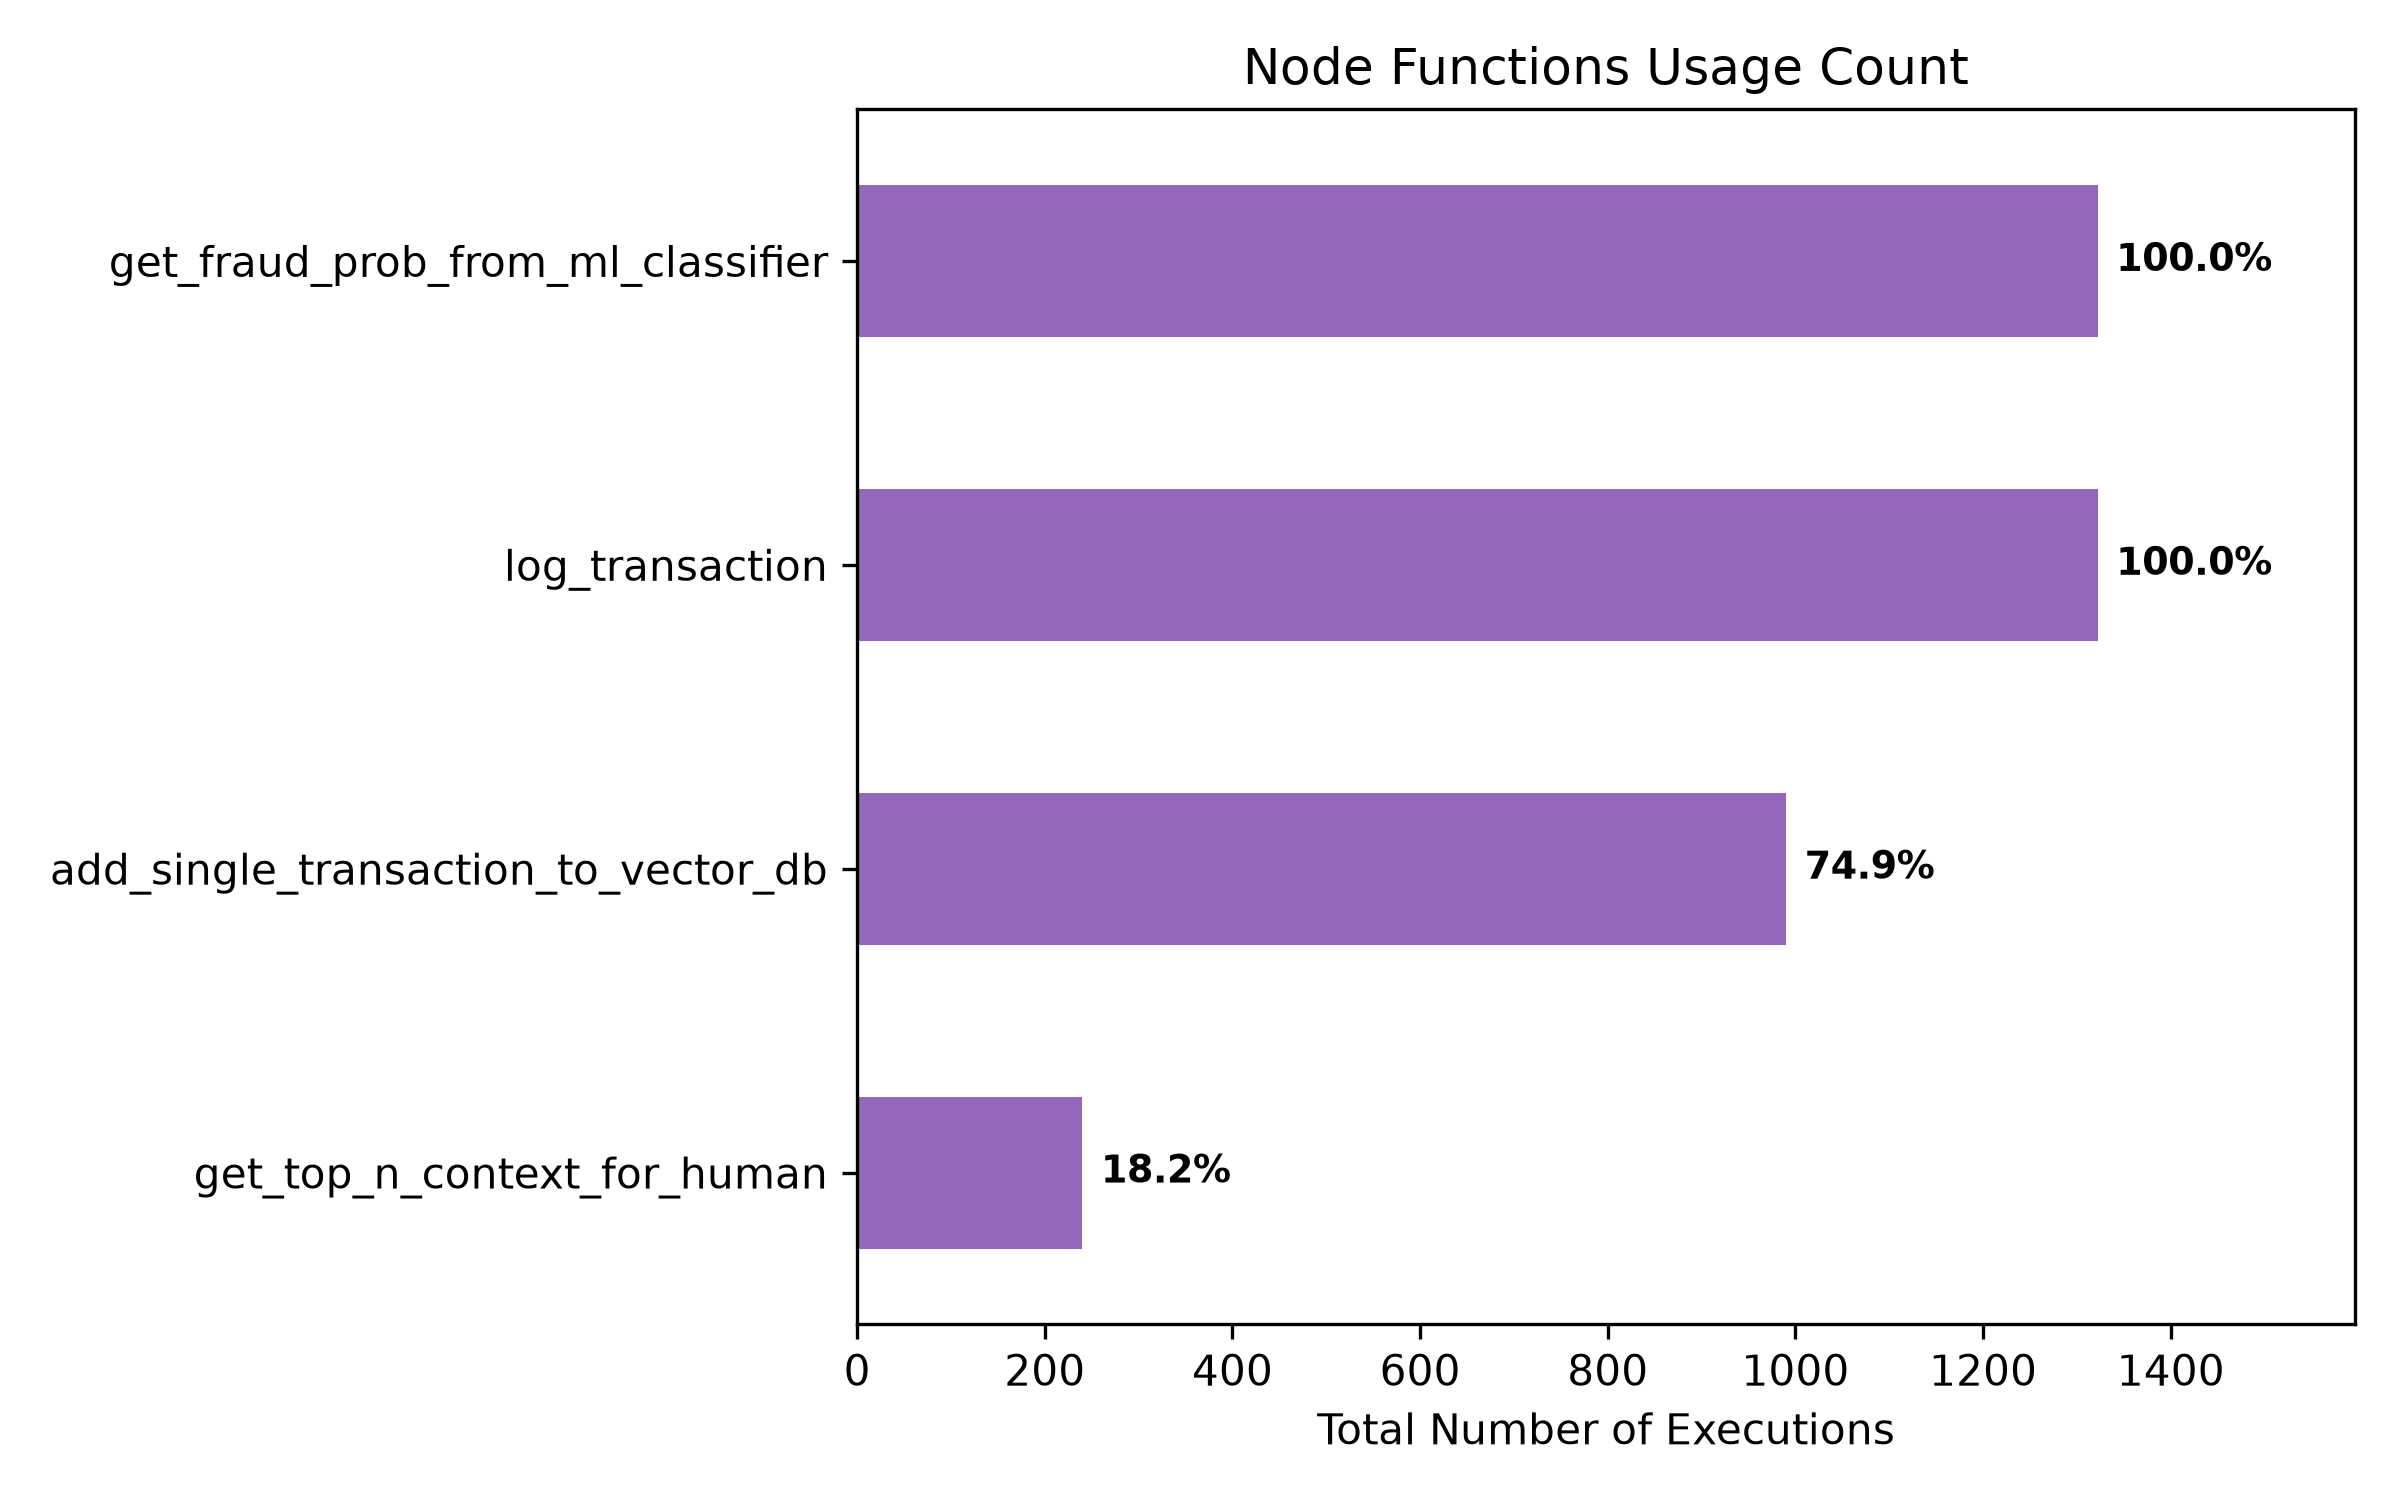
\includegraphics[width=\textwidth]{func_usage.png}
		%\caption{Third Plot ($e^{-x}$)}
		\label{fig:plot3}
	\end{subfigure}
	\hfill
	% Bottom-right subplot
	\begin{subfigure}[b]{0.48\textwidth}
		\centering
		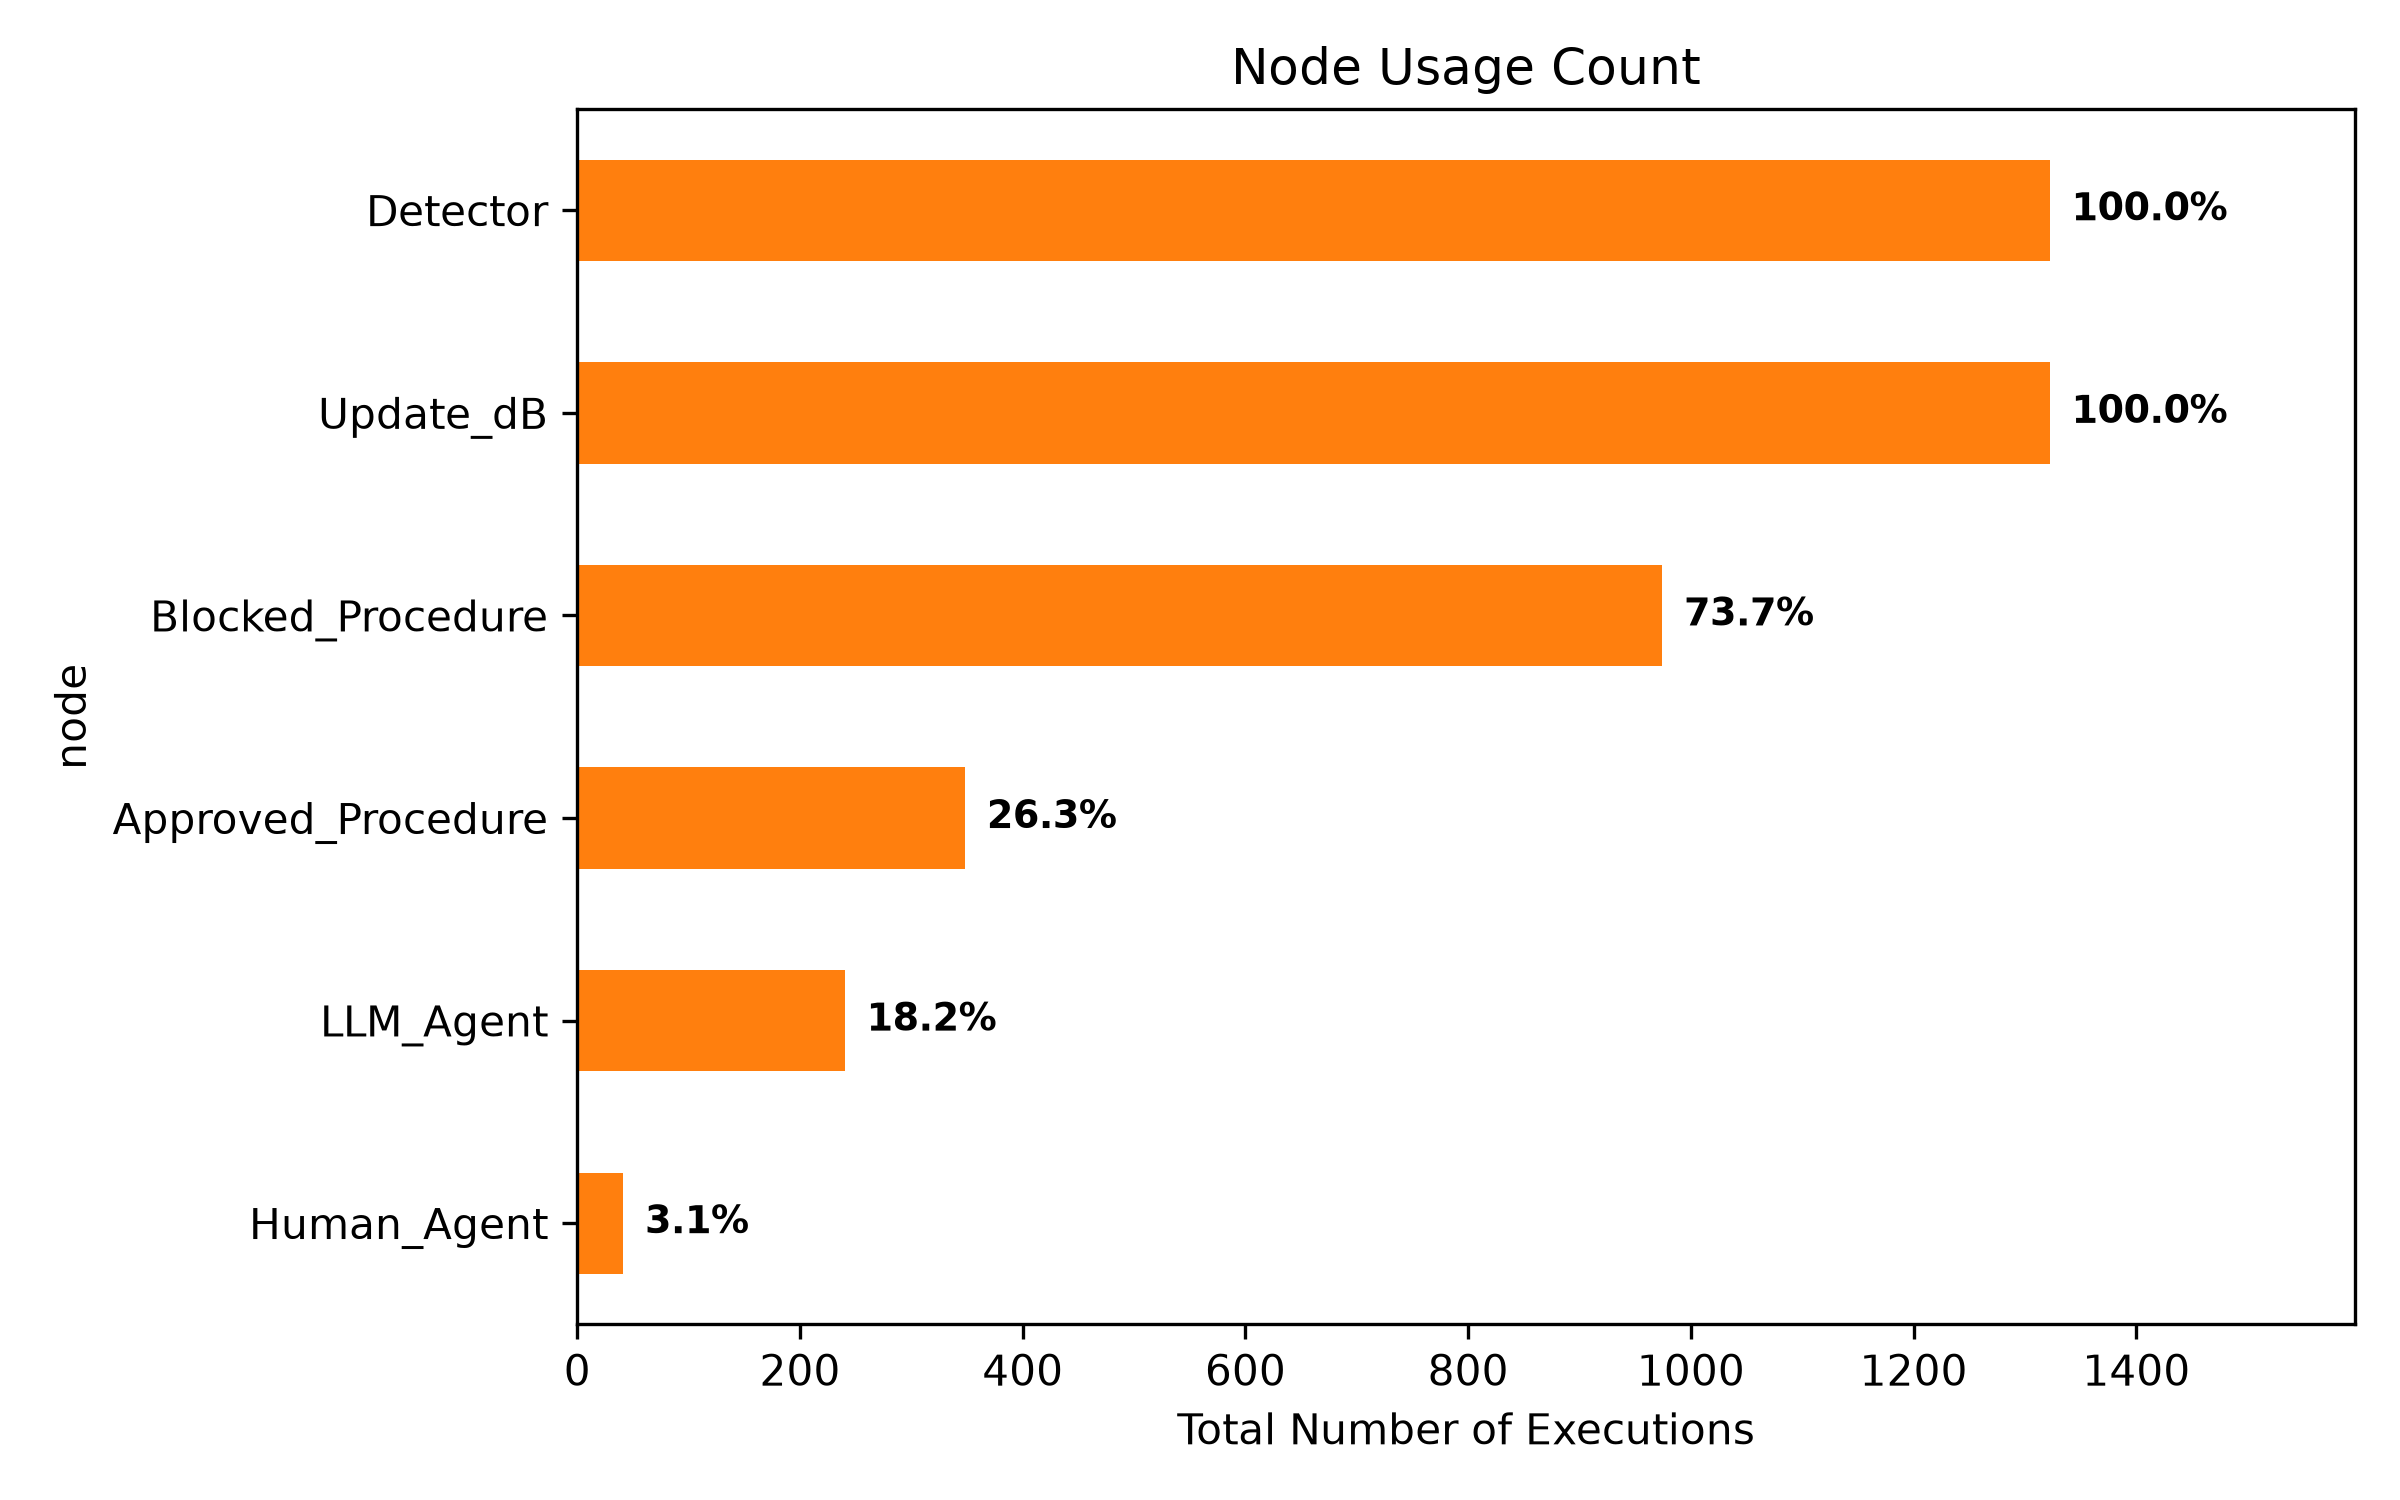
\includegraphics[width=\textwidth]{node_usage.png}
		%\caption{Fourth Plot ($\tan(x)$)}
		\label{fig:plot4}
	\end{subfigure}
	
	\caption{Token, Tool, Function, and Node Usage Analytics.}
	\label{fig:analytics}
\end{figure}

It's worth to emphasize the following regarding node-usage:
\begin{itemize}
	\item  LLM was only involved in 18.2\% of all interactions
	\item  Human involved in 3.1\% of all interactions or $\frac{3.1}{18.2}\approx 17\%$ of LLM interaction.
	%\item  which means LLM Escalate and involved Human in $3.1/18.2\approx 0.17 (17\%)$ of its interactions
\end{itemize}

\section{Professional Relevance}
This project demonstrates end-to-end engineering readiness for modern AI roles by successfully bridging traditional predictive modeling, generative data augmentation, and agentic orchestration frameworks (LangGraph). It highlights a practical capability to design cost-aware enterprise systems that balance automated scale with human-in-the-loop safety.

\section{Future Extensions or Improvements}
\begin{enumerate}[font=\large\color{red}]
	\item Refine the dual-threshold cost function by decoupling distinct agent precision and recall parameters based on production error distributions.
	\item Deploy real-time feedback loops to continuously update the vector database LTM with live verified outcomes.
	\item Expand automated evaluation suites to test resilience against evolving, adversarial fraud patterns.
	\item To avoid possible data leakage due to usage of same data in both step-1: ML-classifier and step-2: Generative model, in production, with the assumption of at least 400-500 samples for robust training of generative model	and 200 samples for final agentic test, we need at least 1200 minority samples, then we can divide dataset into 3 splits of 500 for step-1 (400 for training), 500 for step-2, and 200 for final test. Also this split need to be done properly using stratification on continuous data which has its own challenge (we may need to use quantile-based discretization  prior to stratification).
\end{enumerate}

%\section{Overview and Industry Context}
%Describe the industry problem and why it matters.
%
%\section{Integration Rationale}
%Explain why the selected AI methods were combined and how prior projects informed your design.
%
%\section{System Design and Technical Decisions}
%Describe the system architecture, workflows, and key technical choices (Technical Design Decisions and Tradeoffs)
%
%\section{Ethical Considerations and Responsible AI}
%Analyze ethical risks, bias, transparency, accountability, and safeguards specific to the industry and system.
%
%\section{Evaluation and Reflection}
%Discuss what worked, what did not, and what you learned from integrating across domains.(Limitations and Risks)
%
%\section{Professional Relevance}
%Explain how this work demonstrates readiness for real-world AI roles.(Professional and Industry Relevance)
%
%\section{Future Extensions or Improvements}

%\section{References-x}
%Include all cited sources using a consistent citation style.
%Citations are required when referencing technical concepts, ethical frameworks, or best practices. Do not cite your own results or artifacts.

% apa does not include ref and appx in TOC we forced it
\phantomsection % Ensures hyperref links to the correct page
\addcontentsline{toc}{section}{References}
\printbibliography %[heading=none] % Removes default unnumbered header so it doesn't double-up

% Appendices start here (AFTER references)
% \appendix
% \phantomsection
% \addcontentsline{toc}{section}{Appendix A: Evaluation Metrics for Binary Classification}
% \section{Appendix A: Evaluation Metrics for Binary Classification}\label{app:a}
% When we have a binary classification, we call the classes as positive and negative, for example in our fraud detection, the fraud is positive, and Not-Fraud is the negative class.
% \subsection{Confusion Matrix}
% based on the prediction we can have the following four cases in a table  called confusion matrix as it shown in Table~\ref{tab:conf-mat-def}.
% \begin{table}[!htb]
% 	\centering
% 	\caption{Confusion Matrix}
% 	\label{tab:conf-mat-def}
% 	\begin{tabular}{cc|c|c|}
% 		& \multicolumn{1}{c}{} & \multicolumn{2}{c}{\textbf{Predicted}} \\
% 		& \multicolumn{1}{c}{} & \multicolumn{1}{c}{\textbf{Negative}} & \multicolumn{1}{c}{\textbf{Positive}} \\
% 		\cline{3-4}
% 		\multirow{2}{*}{\textbf{Actual}} & \textbf{Negative} & TN & FP \\
% 		\cline{3-4}
% 		& \textbf{Positive} & FN & TP \\
% 		\cline{3-4}
% 	\end{tabular}
% \end{table}

% \begin{description}
% 	\item [True Positive (TP):] Model correctly predicts the positive class.
% 	\item [True Negative (TN):] Model correctly predicts the negative class.
% 	\item [False Positive (FP):] Model incorrectly predicts the positive class (Type I error).
% 	\item[False Negative (FN):] Model incorrectly predicts the negative class (Type II error).
% \end{description}

% \subsection{Core Binary Classification Metrics}
% Based on the above values, we can define following evaluation metrics
% $$Accuracy =\frac{TN+TP}{TN+TP+FN+FP}$$

% $$Precision = \frac{TP}{TP + FP}$$

% $$Recall = \frac{TP}{TP + FN}$$

% $$False Positive Rate Formula: FPR = \frac{FP}{FP + TN}$$

% $$F1 = 2 \times \frac{Precision \times Recall}{Precision + Recall} = \frac{2TP}{2TP + FP + FN}$$

% $$F_\beta = (1 + \beta^2) \times \frac{Precision \times Recall}{(\beta^2 \times Precision) + Recall}$$

% $$F_\beta = \frac{(1 + \beta^2) \cdot TP}{(1 + \beta^2) \cdot TP + FP + \beta^2 \cdot FN}$$
% \begin{itemize}
% 	\item $\beta > 1$ (e.g., $F_2$): Gives more weight to Recall than Precision.
% 	\item $\beta < 1$ (e.g., $F_{0.5}$): Gives more weight to Precision than Recall
% 	\item $\beta = 1$: Reduces directly to the standard F1-score.
% \end{itemize}

% \subsection{Probability \& Threshold-Based Metrics}
% Generally predictive models produce a probabilities of the classes, and then (in binary classification) using a default thresholds 0.5 then decide the class as 0 or 1. However it's possible to test different thresholds and check the performance, or consider an average base on different threshold as another general performance. There are two important metric in this category (see more details in \parencite{enwiki:roc}):
% \begin{description}
% 	\item[ROC Curve (Receiver Operating Characteristic Curve):] A graphical plot that illustrates the diagnostic ability of a binary classifier system as its discrimination threshold is varied. It plots the True Positive Rate (Recall) on the y-axis against the False Positive Rate (FPR) on the x-axis.
% 	\item[AUC (Area Under the ROC Curve):]  Quantifies the overall ability of the model to discriminate between positive and negative classes across all possible classification thresholds.Interpretation:
% 	\begin{itemize}
% 		\item  $AUC= 1.0$: Perfect classifier.
% 		\item $AUC = 0.5$: Random guessing (no discriminative power).
% 		\item $AUC < 0.5$: Worse than random guessing (often indicates inverted labels)
% 		\item Advantage: Threshold-independent; it measures quality regardless of the chosen decision threshold (e.g., 0.5).
% 	\end{itemize}
% 	\item  [Precision-Recall (PR) Curve, and PR-AUC] A precision-recall curve is a graphical plot that evaluates a binary classification model or information retrieval system by showing the trade-off between precision and recall across different decision thresholds. The AUC for this graph called PR-AUC. A higher area under the curve indicates a better-performing model, especially useful when dealing with heavily imbalanced datasets (such as fraud detection or rare disease screening) where the positive class is rare.

% \end{description}

%ROC Curve (Receiver Operating Characteristic Curve)A graphical plot that illustrates the diagnostic ability of a binary classifier system as its discrimination threshold is varied. It plots the True Positive Rate (Recall) on the y-axis against the False Positive Rate (FPR) on the x-axis.False Positive Rate Formula: $FPR = \frac{FP}{FP + TN}$AUC (Area Under the ROC Curve)Quantifies the overall ability of the model to discriminate between positive and negative classes across all possible classification thresholds.Interpretation:$\text{AUC} = 1.0$: Perfect classifier.$\text{AUC} = 0.5$: Random guessing (no discriminative power).$\text{AUC} < 0.5$: Worse than random guessing (often indicates inverted labels).Advantage: Threshold-independent; it measures quality regardless of the chosen decision threshold (e.g., 0.5).
%%\end{document}

%\newpage
%
%\phantomsection
%\addcontentsline{toc}{section}{Appendix B: XXX}
%\section{Appendix B: XXX}
%Content of Appendix B...
\end{document}


%root@texliveh:/home/dev/xx/zc07-ml-genai-agentic/report/latex/tex# texcount -total report.tex
%Total
%Words in text: 1999
%Words in headers: 54
%Words outside text (captions, etc.): 80
%Number of headers: 12
%Number of floats/tables/figures: 14
%Number of math inlines: 2
%Number of math displayed: 0
%
%root@texliveh:/home/dev/xx/zc07-ml-genai-agentic/report/latex/tex# 


